\documentclass[a4paper,12 pt]{report}
\usepackage{latexsym}
\usepackage[utf8]{inputenc}
\usepackage[T1]{fontenc}

\usepackage[italian]{babel}


\usepackage{graphicx}
\usepackage{hyperref}
\usepackage[table,xcdraw]{xcolor}
\usepackage{setspace}
\usepackage{amssymb}
\usepackage{listings}
\usepackage{url}

\usepackage{xcolor}
\newcommand\myworries[1]{\textcolor{red}{#1}}
 
\usepackage{verbatim}

% The length marginparwidth is less than 2cm and will most likely cause issues with the appearance of inserted todonotes.
\setlength {\marginparwidth }{2cm}

\usepackage{enumitem}
\usepackage{float}
\usepackage{hyperref}
\usepackage{tikz}
\usepackage{multirow}
\usepackage{todonotes}
\usepackage{amsmath, amssymb}
\usepackage{placeins}

\usepackage{amsthm}

\usepackage{graphicx}  
\usepackage{array}
\usepackage{booktabs} 
\usepackage{pifont}
\newcommand{\xmark}{\ding{55}}
\newcommand{\cmark}{\ding{51}} 

\usepackage[square,numbers]{natbib}

% package italiano
%
% Opzionale

\renewcommand{\contentsname}{Sommario}
\renewcommand{\listfigurename}{List of Figures}
\renewcommand{\listtablename}{List of Tables}
\renewcommand{\bibname}{Bibliografia}
\renewcommand{\indexname}{Indice}
\renewcommand{\figurename}{Figura}
\renewcommand{\tablename}{Tavola}
\renewcommand{\partname}{Parte}
\renewcommand{\chaptername}{Capitolo}
\renewcommand{\appendixname}{Appendice}
\renewcommand{\abstractname}{Abstract}
\renewcommand{\footnotesize}{\scriptsize}
\renewcommand{\today}{\ifcase\month\or
  Gennaio\or Febbraio\or Marzo\or Aprile\or Maggio\or Giugno\or
  Luglio\or Agosto\or Settembre\or Ottobre\or Novembre\or Dicembre\fi
  \space\number\day, \number\year}

% package formato
\pagestyle{plain}
\setlength{\topmargin}{0.0in}
\setlength{\headheight}{0.0in}
\setlength{\headsep}{0.0in}
\setlength{\footskip}{0.5in}
\setlength{\textheight}{8.5in}
\setlength{\textwidth}{6in}
\setlength{\oddsidemargin}{0.25in}
\setlength{\evensidemargin}{0.25in}
\setlength{\parindent}{0.4 in}
\onehalfspacing


\def\cent{\centerline}
\def\vs{\vskip 10 pt plus 1 pt}
\def\bs{\bf}
\def\grad{\vec{\nabla}}
\def\gradx{\vec{\nabla}_x}
\def\epsilon{\varepsilon}

\newtheorem{theorem}{Theorem}[section]
\newtheorem{corollary}{Corollary}[theorem]
\newtheorem{lemma}[theorem]{Lemma}

\newtheorem{lemm}{Lemma}[chapter]
\newtheorem{proposizion}[lemm]{Proposizione}
\newtheorem{teorem}[lemm]{Teorema}
\newtheorem{corollari}[lemm]{Corollario}
\newtheorem{esempi}[lemm]{Esempio}

\newcommand{\cvd}{\begin{flushright}$\Box$\end{flushright}}
\newcommand{\tr}{{\rm Tr}\;}
\newcommand{\eq}{\begin{equation}}
\newcommand{\feq}{\end{equation}}
\theoremstyle{definition}
\newtheorem{definition}{Definition}[section]
 
\theoremstyle{remark}
\newtheorem*{remark}{Remark}

\definecolor{blu_dmi}{HTML}{002e62}


% reset del counter dei chapter, divisore table of contents
\makeatletter
  \@addtoreset{chapter}{part}
\makeatother 
%%%%%%%%%%%%%%%%%%%%%%%%%%%%%%%%%
%%%%%%%%%%%%%%%%%%%%%%%%%%%%%%%%%
%%%%%%%%%%%%%%%%%%%%%%%%%%%%%%%%%
%%%%%%%%%%%%%%%%%%%%%%%%%%%%%%%%%



\begin{document}
    % Thesis frontmatter --------------------------------------------

\thispagestyle{empty} %suppress page number

	\noindent % just to prevent indentation narrowing the line width for this line
	
\includegraphics[width=0.15\textwidth]{img/logoUniPg}
	\begin{minipage}[b]{0.7\textwidth}
		\centering
		{\Large{\textsc{Universit{\`a} di Perugia}}}\\
		\vspace{0.4 em}
		{\large {Dipartimento di Matematica e Informatica}}
		\vspace{0.6 em}
	\end{minipage}%
	
\includegraphics[width=0.15\textwidth]{img/logoDMI}
	
	\vspace{8 em}

	\begin{center}
		

	
		{\Huge{Appunti Knowledge Representation and Automated Reasoning }}\\
		\vspace{2 em}
		{\large { Autore: Chiara Luchini}}\\
		\vspace{5 em}
		{\large {Basati su:}}\\
		{\large {- Slides del Prof. Stefano Bistarelli}}\\
		{\large {- Lezioni del Prof. Stefano Bistarelli}}\\
		%{\large \textcolor{blu_dmi}{- Appunti lezioni online Prof. Alfredo Navarra}}\\
		
	
	

%		\makebox[380pt][c]{\textcolor{blu_dmi}{\textit{Advisor} \hfill \textit{}}}
%		\makebox[380pt][c]{\textcolor{blu_dmi}{\textbf{Dott. Francesco Santini \hfill}}}
		
		\vspace{6 em}
		\vfill
		
	{\rule{380pt}{.4pt}}\\
		\vspace{1.2 em}
		\large{{Anno Accademico 2021/2022}}
		
		
		
		
	\end{center}

% ------------------------------------------------------------------
     \tableofcontents
    % Opzionale
    \newpage
    \thispagestyle{empty} %suppress page number

\chapter*{Libri di riferimento}
\section*{Libri per appunti Prof.Bistarelli}
\begin{itemize}
    \item Computer Security: Principles and Practice, Global Edition \cite{comp_sec_principles}
\end{itemize}


\section*{Libri per appunti Prof.Santini}
\begin{itemize}
    \item Secure Coding in C and C++ \cite{secure_coding_c}
\end{itemize}

    \newpage
    
    % Parte Santini
    \part{Appunti parte Prof. Santini}
    \chapter{Alcune terminologie}
\label{ch:terminologie}
In questo Capitolo verranno riportate alcune delle terminologie utilizzate nel campo della Cybersecurity.

\section{Security Flaws}
Una \textbf{falla} o \textbf{difetto della sicurezza} è un difetto del software che rappresenta un potenziale rischio per la sicurezza. Quest'ultimo può essere visto come la codifica di un errore umano nel software incluse le omissioni, infatti un difetto del software può originarsi in ogni momento del ciclo di vita di questo. Ovviamente non tutti i difetti nel programma sono delle falle di sicurezza, quelli che lo sono devono essere rilevati ed eliminati in modo da evitare potenziali attacchi. Questa premessa sottolinea la relazione tra ingegneria del software e sicurezza del programma. Un aumento della qualità nella scrittura del codice porta anche a un aumento della sicurezza. Tuttavia, molte falle di sicurezza non vengono rilevate perché processi di sviluppo software tradizionali raramente considerano l'esistenza di aggressori.

\section{Vulnerabilità}
Una \textbf{vulnerabilità} è un insieme di condizioni che permetto all'attaccante di violare un policy di sicurezza esplicita o implicita. Una falla nella sicurezza di un programma può rendere il software vulnerabile agli attachi quando i dati in input superano un limite di sicurezza.\\
Ciò può verificarsi quando un programma contenente una falla è installato con privilegi di esecuzione maggiori di quelli della persona che lo esegue o è utilizzato da un servizio di rete dove i dati in input arrivano tramite la connessione a internet.

\subsection{Le falle non sono vulnerabilità}
Una falla può esistere senza tutte le precondizioni necessarie a creare una vulnerabilità. Viceversa una vulnerabilità può esistere senza una falla. Poichè essendo la sicurezza un attributo di qualità che deve essere scambiato con altri come ad esempio le performance e l'usabilità, i designer di software possono intenzionalmente lasciare i loro prodotto vulnerabile per alcune forme di exploit. Ciò significa che il designer ha accettato il rischio per conto del consumatore.

\section{Policy}
Una \textbf{policy di sicurezza} è un insieme di regole e pratiche che speficano o regolano come un sistema o un organizzazione fornisce dei servizi di sicurezza per proteggere delle risorse di sistema sensibili e critiche. Coloro che sono documentate, ben conosciute, e visibilmente imposte possono aiutare a stabilire il comportamento dell'utente.

\section{Exploit}
L'\textbf{exploit} è una tecnica che trae vantaggio di una vulnerabilità di sicurezza per violare un policy di sicurezza esplicita o implicita. Le vulnerabilità sono soggette a sfruttamento, gli exploit possono essere di diverso tipo dai worms ai virus fino ad arrivare ai trojan. Una buona compresione di come il programma può essere sfruttato è un valido strumento da utilizzare per sviluppare un software sicuro.

\section{Zero-day exploit}
Una vulnerabilità \textbf{zero-day o 0-day} è una vulnerabilità del software-computer che è sconosciuta a coloro che sarebbero interessati nel mitigare quest'ultima, incluso il fornitore del software.  Un exploit mirato a un zero-day è chiamato \textbf{zero-day exploit o zero-day attack}.

\section{Mitigazioni}
La \textbf{mitigazione} racchiude i metodi, tecniche, processi, strumenti, o librerie di runtime che possono prevenire o limitare gli exploit contro le vulnerabilità.
Una mitigazione o contromisura è una soluzione per le falle o una soluzione alternativa che può essere applicata per prevenire l'exploit. Esempi:
\begin{itemize}
    \item A livello di codice sorgente: una mitigazione può essere una semplice sostituzione di un'operazione di string copy illimitata con un limitata;
    \item A livello di sistema o network: una mitigazione può coinvolgere lo spegnimento di una porta o il filtraggio del traffico per prevenire un attacco.
\end{itemize}
\subsection{Gestione delle falle e delle vulnerabilità}
Il metodo preferito per eliminare una falla è di trovare il difetto e correggerlo. Tuttavia, in alcuni casi è più conveniente eliminare le falle prevenendo l'utilizzo di input dannosi nel difetto. Un altro modo di gestire le vulnerabilità consiste nell'isolamento di quest'ultima, ovviamente affrontandola operativamente ne aumenta il costo della mitigazione poichè esso viene spostato dallo sviluppatore agli amministratori di sistema e agli utenti finali.

\section{Collegamento con CIA}
Una risorsa fisica o logica può avere una o più vulnerabilità che possono essere sfruttate da un attaccante. Il risultato può compromettere potenzialmente la \textbf{confidenzialità}, l'\textbf{integrità} o la \textbf{disponibilità} delle risorse.

\chapter{Linguaggio C}
Il linguaggio di programmazione C è conosciuto per essere un linguaggio leggero con un numero di "tracce" ridotto.
Alcuni programmatori abituati ad usare altri linguaggi come Java, Pascal o Ada credono che il linguaggio li protegga di più rispetto a quello che effettivamente fa. Queste false ipotesi hanno portato i programmatori a fallire nel prevenire la scrittura di un array oltre i limiti, fallire nel rilevare overflow di interi e anche nel chiamare funzioni con un numero errato di parametri.

\section{CERT C coding standard}
Il SEI CERT C Coding Standard è una codifica standard per i software per il linguaggio di programmazione C, sviluppato da il CERT Coordination Center per migliorare la sicurezza, l'affibidabilità del sistema di software.

\section{Tipi di dato e Interi}
I tipi \verb|int| sono rappresentati dall'insieme dei numeri naturali, incluso lo $0$, ($0, 1, 2, 3, ...$) uniti
ai numeri naturali negativi ($-1, -2, -3, ...$). In C sono presenti vari tipi di interi come mostrati nella tabella sottostante:

\begin{figure}[H]
    \centering
    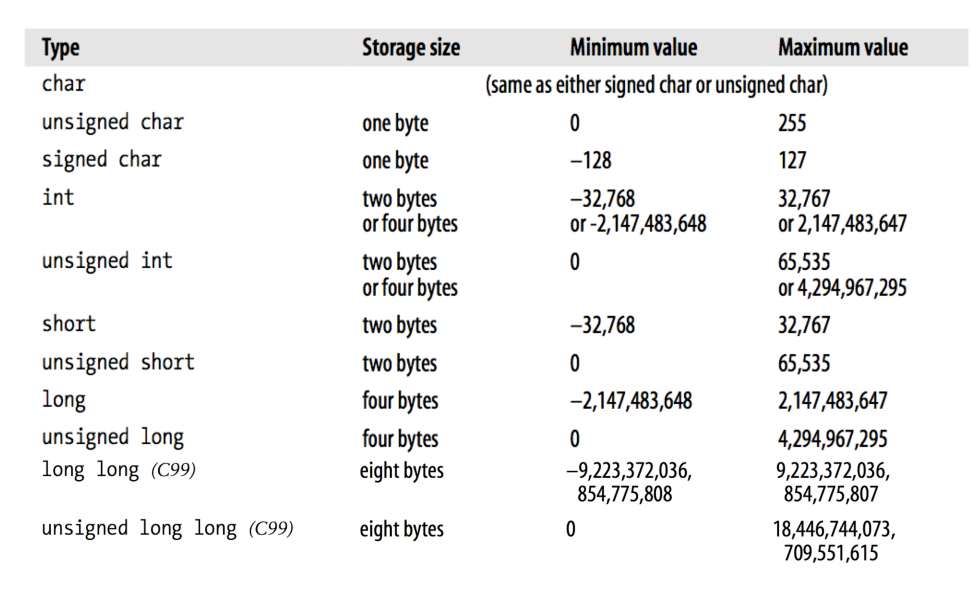
\includegraphics[width=13cm, keepaspectratio]{capitoli/secure_coding/img/cap_2/vari_tipi.png}
    \caption{Tabella raffigurante tutti i tipi in C con la loro dimensione.}\label{fig:vari_tipi}
\end{figure}

I numeri interi con segno (\verb|signed int|) sono ottenuti utilizzando il \textbf{complemento a 2}, che permette di rappresentare sia numeri positivi
che negativi utilizzando 1 bit per il segno (il primo bit) e risolvendo il problema del doppio 0 aggiungendo 1 dopo aver fatto il complemento bit a bit.
Rappresentando 8 bit con il complemento a 2 avremmo un range che varia tra $-128$ a $127$.
In generale il range di rappresentazione sarà dato dalla seguente formula:
\[
    da \ -2^{N} - 1 \ \ a \ \ 2^{N - 1} - 1
\]

dove $N$ è il numero di bit.

%%TODO: aggiungere wraparound

\section{Vulnerabilità degli Interi}

I potenziali probelmi alla sicurezza causati dagli int provengono da errori di 3 tipi:

\begin{itemize}
    \item \textbf{Overflow/Wraparound}: occorre quando un'operazione genera valori
          che si trovano al di fuori del range di un particolare tipo di interi
    \item \textbf{Truncation}: occorre quando un valore viene salvato in un tipo
          troppo piccolo per rappresentarlo
    \item \textbf{Conversions}: sono errori generati da cast impliciti o espliciti
          in valori che si trovano al di fuori del range del tipo risultante.
\end{itemize}

Ci sono vari modi per prevenire tali errori:

\begin{itemize}
    \item \textbf{Integer Type Selection}:
          consiste nel selezionare il tipo più
          appropriato per il codice che si ha sotto mano.
          Un esempio è l'uso del tipo \verb|size_t| quando si vuole salvare la dimensione di un oggetto dato che ideato per questo scopo
          ("INT01-C. Use \verb|size_t| for all integer values representing the size of
          an object.").
          Si può anche utilizzare \verb|short|.\\
          Un esempio: \verb|size_t total = strlen(argv[1])+ 1;|
    \item \textbf{Type Range Checking}:
          controlla se avvengono errori legati al superamento del range degli interi,
          alcuni modi per farlo solo: \begin{itemize}
              \item \textit{Pre-Conditions}:
                    questa tecnica si basa sul controllare la possibile presenza di
                    overflow o wrapping prima che un'operazione venga eseguita.
                    Di seguito un esempio:
                    \begin{lstlisting}
unsigned int ui1, ui2, usum;

// initialize ui1 and ui2

if (UINT_MAX - ui1 < ui2) {
    // handle error condition
}
else {
    usum = ui1 + ui2;
}
                    \end{lstlisting}
              \item \textit{Post-Conditions}:
                    è equivalente alla pre-condition ma viene eseguita dopo
                    l'esecuzione di un'operazione ed è in grado di controllare solo la
                    presenza di wrapping. Di seguito un esempio:
                    \begin{lstlisting}
    unsigned int ui1, ui2, usum;

    // initialize ui1 and ui2

    usum = ui1 + ui2;

    if (usum < ui1) {
        // handle error condition
    }
                    \end{lstlisting}
          \end{itemize}
    \item \textbf{Secure Integer Libraries}:
          sono presenti librerie sviluppate appositamente per gestire questi
          tipi di errori tramite meccanismi architecture-specific.
    \item \textbf{Compiler Checks}:
          GCC fornisce il flag \verb|-ftrapv| che crea delle trap per le
          operazioni di addizione, sottrazione e moltiplicazione con segno
          quando generarno overflow a runtime.
    \item \textbf{Testing e Static Analysis}:
          effettuare procedure di Static Analysis,
          dal compilatore o un altro stumento apposito,
          per la detection di possibili errori nei range degli itneri.
\end{itemize}

\section{Array e stringhe}
\paragraph{Problemi con gli array.}Il  CERT C Secure Coding Standard include il fatto di non applicare l'operatore \textit{sizeof} a un puntatore wuando si vuole la grandezza dell'array.
Esempio:
\begin{figure}[H]
    \centering
    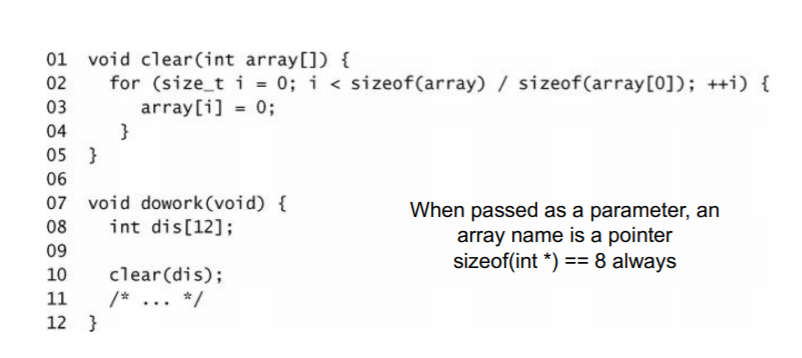
\includegraphics[width=10cm, keepaspectratio]{capitoli/secure_coding/img/cap_2/sizeof_array.png}
    \caption{Esempio \textit{sizeof(array)} .}\label{fig:sizeof_array}
\end{figure}
\paragraph{Stringhe.} Le stringhe sono un concetto fondamentale nell'ingegneria del software, ma essi non sono un tipo integrato in C o C++. Infatti la libreria standard di C supporta le stringhe di tipo \verb|char| e le stringhe larghe di tipo \verb|wchar_t|.
\begin{figure}[H]
    \centering
    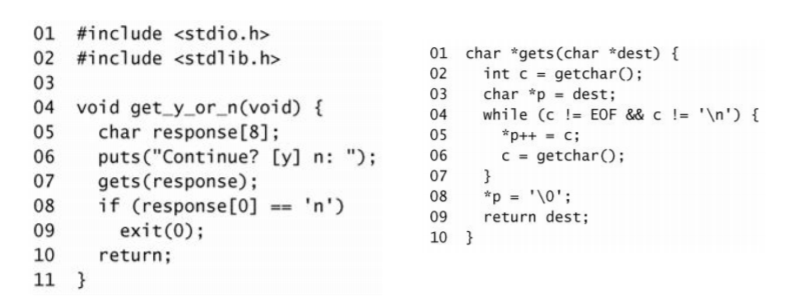
\includegraphics[width=10cm, keepaspectratio]{capitoli/secure_coding/img/cap_2/gets_1.png}
    \caption{Esempio \textit{gets} .}\label{fig:gets}
\end{figure}
Il problema principale con la funzione \verb|gets()| è che non fornisce alcun modo di specificare un limite sul numero dei caratteri da leggere.
Quest'ultima risulta deprecata e eliminata, il CERT consiglia di non utilizzare funzioni deprecate o obsolete.

\paragraph{Lettura da \textit{stdin()}.} La lettura dei dati da una una fonte illimitata come \textbf{stdin()} crea dei problemi per il programmatore poiché non è possibile conoscere in anticipo quanti caratteri un utente utilizzerà, infatti è impossibile pre-allocare un array di sufficiente lunghezza. Una soluzione comune è di allocare staticamente un array più grande rispetto al necessario. Questo approccio funziona con gli utenti "amichevoli", ma con gli attaccanti un array di caratteri di lunghezza fissa può essere facilmente superato. Infatti questo metodo è probito dal CERT il quale afferma che non si può copiare dati da una fonte illimitata in un array con lunghezza fissata.\\
\textit{“STR35-C. Do not copy data from an unbounded
    source to a fixed-length array.”}
\paragraph{Parametri dei programmi.} Le vulnerabilità possono occorrere quando uno spazio indeguato è allocato per copiare un input di un programma come un argomento della riga di comando.

\begin{figure}[H]
    \centering
    
\includegraphics[width=10cm, keepaspectratio]{capitoli/secure_coding/img/cap_2/parametri_funzioni.png}
    \caption{Esempio vulnerabilità con parametri dei programmi .}\label{fig:parametri_programmi}
\end{figure}
Nonostante \verb|argv[0]| contiene il nome del programma, un attaccante può controllare il contenuto di \verb|argv[0]| per causare una vulnerabilità fornendo una stringa con più di 128 bytes.

\paragraph{Null terminating string.}
In Figura \ref{fig:null_string} possiamo vedere che il risultato di \verb|strcpy()| su c porta l'utente a poter scrivere oltre i limiti dell'array poichè la stringa salvata in \verb|a[]| non terminata correttamente (null-terminating).


\begin{figure}[H]
    \centering
    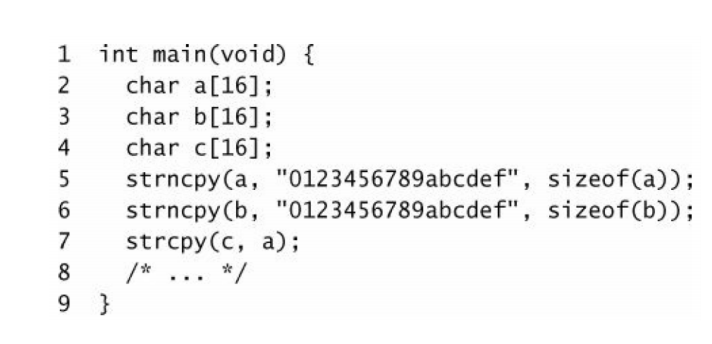
\includegraphics[width=10cm, keepaspectratio]{capitoli/secure_coding/img/cap_2/null_string.png}
    \caption{Esempio null terminating string .}\label{fig:null_string}
\end{figure}
\textit{“STR32-C. Null-terminate byte strings as
    required.”}

\paragraph{Funzionamento esempio \ref{fig:null_string}}
Abbiamo 3 array lunghi 16 caratteri, copiamo la stringa "0123456789abcdef" in \textbf{a} e in \textbf{b}, come si può notare questa stringa ha una lunghezza di 16 caratteri. Successivamente si copia la stringa contenuta in \textbf{a} nell'array \textbf{c} e questo porta ad avere dei problemi ovvero:
\begin{itemize}
    \item non viene salvato sia in \textbf{a} che in \textbf{b} il carattere di fine stringa "\textbackslash0" allora essendo che la stringa non termina e che 'array \textbf{b} è memorizzato subito dopo \textbf{a} si ha di conseguenza che
          \[a = [0123456789abcde0123456789abcde\backslash 0]\]
    \item quindi quando si va a copiare \textbf{a} dentro \textbf{c} si copiano 32 caratteri più "\textbackslash0" e non 16 sforando così la memoria allocata inizialmente.
\end{itemize}
\section{Vulnerabilità delle stringhe ed exploit}
\subsection{Valori corrotti}
Precedentemente abbiamo visto alcuni degli errori più comuni nel manipolare il linguaggio C o C++. Questi errori sono pericolosi nel momento in cui il codice opera con dati esterni non fidati come gli argomenti delle linee di comando, variabili d'ambiente, input della console, file di testo e connessione a internet. \textbf{Infatti è meglio considerare tutti i dati esterni al codice come non fidati. } Nell'analisi della sicurezza dei software, un valore è chiamato \textbf{corrotto (tainted)} quando viene da una risorsa non fidata, al di fuori del controllo del programma, e non \textbf{è stato sanificato} per assicusarsi che sia conferme a qualsiasi vincolo posto su di esso.
\begin{figure}[H]
    \centering
    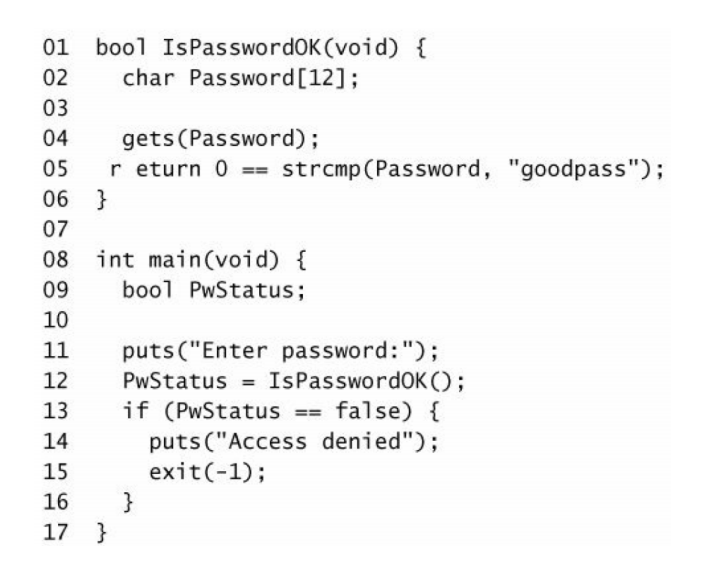
\includegraphics[width=10cm, keepaspectratio]{capitoli/secure_coding/img/cap_2/password_example.png}
    \caption{Esempio password.}\label{fig:password}
\end{figure}

\subsection{Buffer overflow.}
In questo caso la falla sta nella funzione \verb|IsPasswordOk()| poichè permette ad un attaccante di guadagnare l'accesso non autorizzato causato dalla funzione \verb|gets()|. Questa tipologia di attaccco che permette una scrittura oltre i limiti viene definita \textbf{buffer overflow}.

\begin{figure}[H]
    \centering
    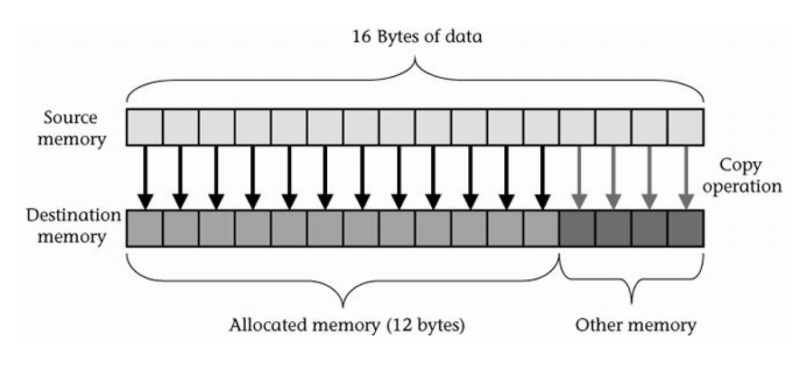
\includegraphics[width=10cm, keepaspectratio]{capitoli/secure_coding/img/cap_2/memory.png}
    \caption{Allocazione della memoria.}\label{fig:memoria}
\end{figure}
Oltre questo è presente anche un altro problema ovvero che il programma \verb|IsPasswordOk| non controlla lo stato di ritorno di \verb|gets|. \\
\textit{“FIO04- C. Detect and handle input and output errors.”}\\
Quando si fallisce l'inserimento della password non viene controllato da nessuno perciò il contenuto del buffer \verb|Password| è indeterminato, nei programmi reali esso potrebbe contenere la password del precedente utente.
Il buffer overflow occorre quando un dato è scritto oltre i limiti della memoria allocata in una particolare struttura. Il linguaggio C e C++ sono suscettibili a questi attacchi poichè:
\begin{itemize}
    \item Definisce le stringhe come array di caratteri con terminazione null;
    \item Non usano dei metodi per il controllo implicito dei limiti;
    \item Fornisce funzioni per le stringhe che non appplicano dei controlli.
\end{itemize}
Non tutti i buffer overflow portano a delle vulnerabilità, solo nel caso in cui un attaccante può manipolare gli input controllati dall'utente per sfruttare una falla di sicurezza.\\
Il buffer overflow può essere sfruttato sia nella memoria \textbf{heap} che in quella \textbf{statica} sovrascrivendo strutture di memoria adiacenti. Per aiutare nel verificare la presenza di un buffer overflow esistono dei programmi che a tempo di compilazione (\textbf{staticamente}) o in modo \textbf{dinamico} (eseguono il programma passando delle stringhe dove viene richiesto) controllano la presenza o meno di quest'ultimi.

\section{Memoria}
\subsection{Organizzazione di un processo in memoria}
Nell'immagine sottostante possiamo vedere come è organizzata la memoria in 3 differenti casi, il primo è il caso generale che andremo a prendere in considerazione, il secondo riguarda la memoria in Linux e l'ultimo in Windows.

\begin{figure}[H]
    \centering
    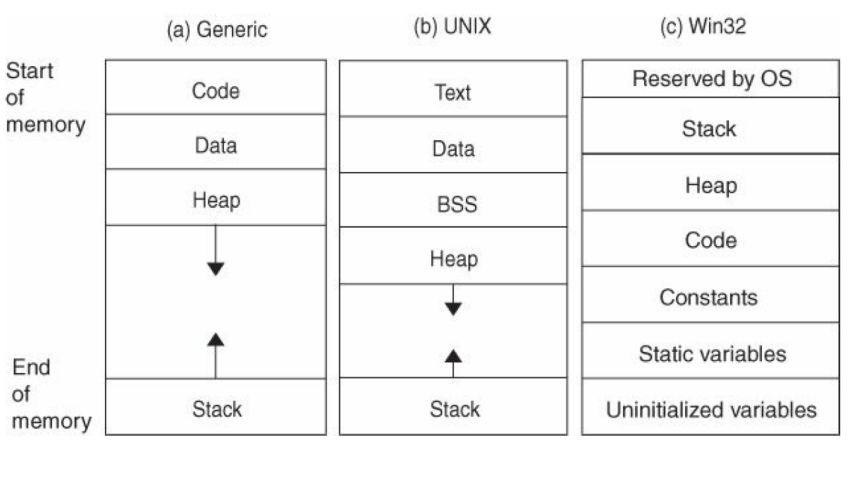
\includegraphics[width=10cm, keepaspectratio]{capitoli/secure_coding/img/cap_2/memoria.png}
    \caption{Organizzazione della memoria.}\label{fig:org_memoria}
\end{figure}
Studiamo le varie parti della memoria nel caso generale:
\begin{itemize}
    \item \textbf{Code}: zona in cui viene salvato il codice del programma;
    \item \textbf{Data}: memoria  in cui sono salvate le variabili globali e le variabili locali statiche, inizializzate e non;
    \item \textbf{Heap:} memoria per allocazione dinamica dei processi, gli indirizzi di memoria aumentano in modo crescente;
    \item \textbf{Stack:} zona LIFO (pila) in cui vengono salvate le variabili locali alle funzioni (supporto per l'esecuzione dei processi), gli indirizzi di memoria aumentano in modo decrescente .
\end{itemize}
Noi vedremo degli esempi di buffer overflow nello stack, è molto importante ricordarsi come funziona e come vengono salvate le variabili, se si alloca dello spazio si va da un numero più alto a uno più basso e viceversa (come una fisarmonica). La memoria è struttura in questo modo così la parte dinamica (heap) non si incontra con la parte statica (stack) a meno che non viene riempita completamente.\\
La memoria UNIX è molto simili alla memoria generale, l'unica differenza sta nel fatto che la parte \textbf{Data} nella memoria generale viene suddivisa in due in quella UNIX:
\begin{itemize}
    \item \textbf{Data:} vengono salvate delle variabili globali/statiche inizializzate;
    \item \textbf{BSS(Block Started by Symbol):} vengono salvate le variabili globali che non sono state inizializzate e vengono di default inizializzate a 0.
\end{itemize}
Il segmento \textbf{Text} è l'equivalente del segmento \textbf{Code}, entrambi includono le istruzioni e i dati read-only.

\paragraph{Esecuzione di un programma.}
Vediamo un primo esempio di esecuzione di un programma. In questo caso possiamo vedere due funzioni \verb|main()| e \verb|fun(...)|, si parte salvando in memoria le variabili locali presenti nella funzione \verb|main()| la quale richiama l'altra. In Figura \ref{fig:es_esec_processo} possiamo vedere che le variabili vengono salvate in sequenza dal basso verso l'alto in base a come sono state inizializzate, successivamente con la chiamata di \verb|fun()| si salvano i parametri che essa prende in input, l'indirizzo di ritorno (\textbf{return address}\footnote{indica l'indirizzo di ritorno dopo che è stata eseguita la funzione in questione, in questo caso indica l'indirizzo del main.}) e la variabile res. Il segmento che contiene la variabile del main si chiama \textbf{stack/frame main}, stessa definizione per il segmento di fun. Al termine dell'esecuzione di fun si cancella dalla memoria tutto quello riguardante quest'ultima e si ritorna all'istruzione successiva alla chiamata di funzione in main. Per riportare il controllo nella posizione corretta, deve essere salvato l'indirizzo di ritorno. Lo stack è adatto a mantenere queste informazioni perché è una struttura dati dinamica in grado di supportare qualsiasi livello di annidamento all'interno vincoli di memoria.
\begin{figure}[H]
    \centering
    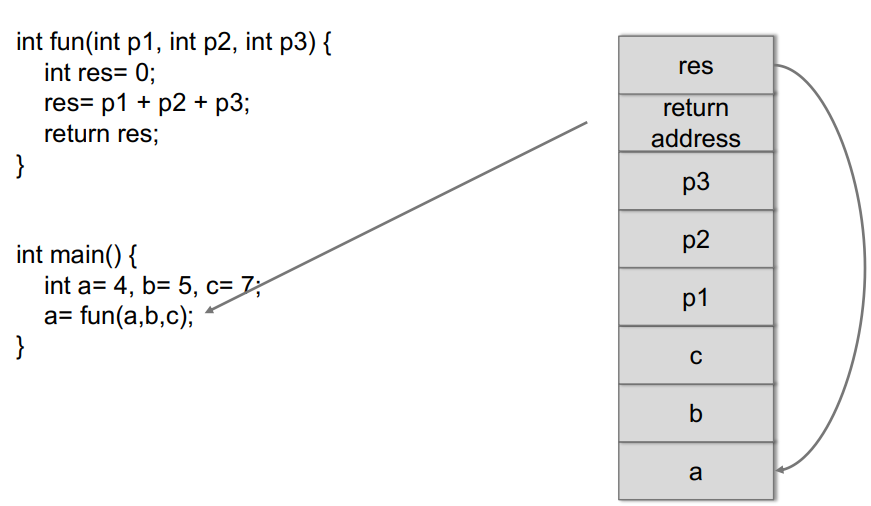
\includegraphics[width=13cm, keepaspectratio]{capitoli/secure_coding/img/cap_2/es_esecuzione_processo.png}
    \caption{Esempio esecuzione processo.}\label{fig:es_esec_processo}
\end{figure}
\subsection{Puntatori}
\subsubsection{Extended base pointer (EBP)}
L'indirizzo del frame corrente è salvato all'interno del frame o nel \textbf{base pointer register}. Il registro \textbf{extended base pointer (ebp) } è usato per questo scopo, esso è usato anche come punto fissato di riferimento all'interno dello stack. Quando una subroutine è chiamata, il puntatore del frame per la routine di chiamata viene anch'esso inserito nello stack in modo che può essere ripristinato quando la subroutine termina.
\subsubsection{Instruction pointer}
Il \textbf{puntatore di istruzione (eip)} punta all'istruzione successiva da eseguire, quando si esegue una sequenza di istruzioni esso è aumentato automaticamente dalla grandezza di ogni istruzioni. Eip non può essere modificato direttamente ma deve essere modificato indirettamente con delle istruzioni come :
\begin{itemize}
    \item jump;
    \item call;
    \item return.
\end{itemize}

\subsubsection{Extended stack pointer (ESP)}
L'\textbf{extended stack pointer (esp)} è il puntatore corrente allo stack, esso punta alla parte superiore della pila.



\section{Stack overflow}
\paragraph{Secondo esempio}
In questo secondo esempio possiamo vedere che ci sono 3 funzioni ( \verb|main|, \verb|f1| e \verb|f2|) che si chiamano a vicenda. Quando viene eseguito il programma viene inserito nello stack il frame del \verb|main|, supponiamo che esso inizi dall'indirizzo 1000, il quale viene salvato all'interno del ebp e del registro della CPU. Successivamente quando viene chiamata la funzione \verb|f1| l'ebp all'interno del registro della CPU cambia con quello dell'inizio del frame di \verb|f1|, ovvero 1008. All'interno del frame di \verb|f1| vengono salvati oltre alle variabili locali anche il valore del ebp corrente(1008) e il valore di ritorno, il quale è uguale all'epb del \verb|main| poiché appena terminata \verb|f1| la CPU deve tornare a eseguire le istruzioni successive alla chiamata di funzione nel frame \verb|main|.
\begin{figure}[H]
    \centering
    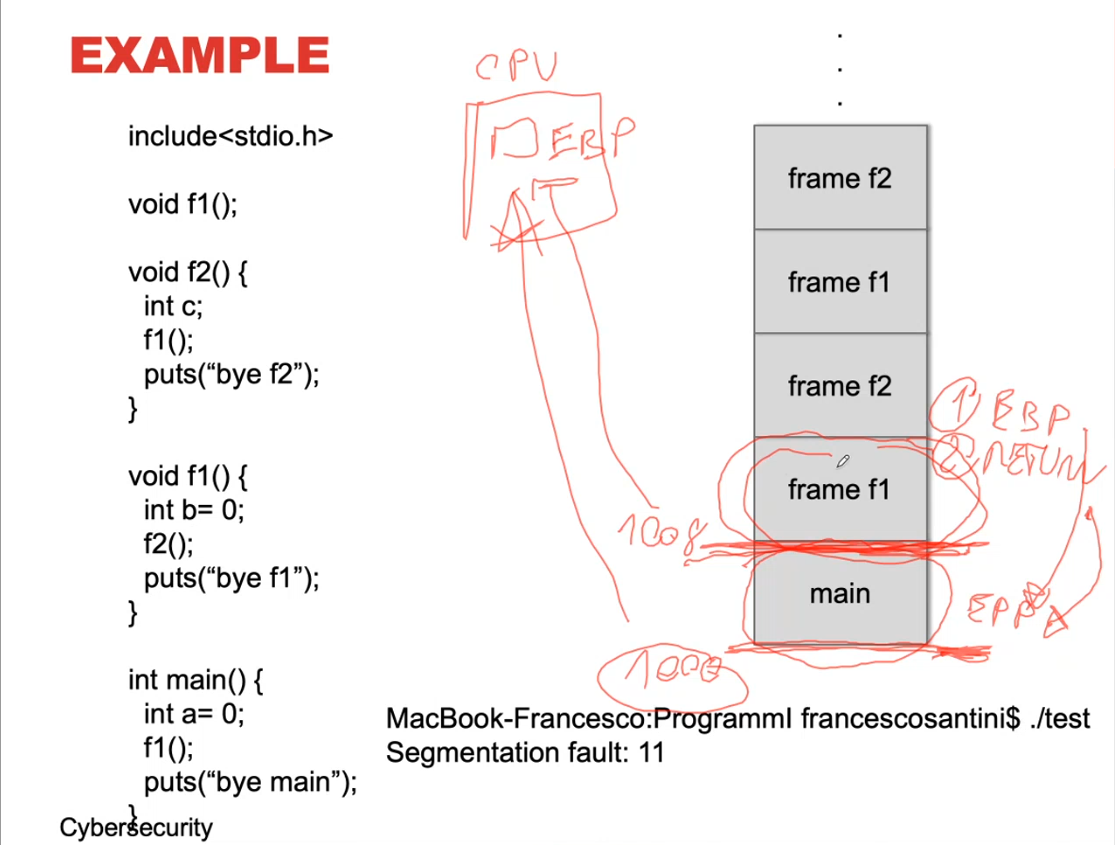
\includegraphics[width=13cm, keepaspectratio]{capitoli/secure_coding/img/cap_2/es_process_spiegato.png}
    \caption{Esempio esecuzione processo con spiegazione.}\label{fig:es_esec_processo2}
\end{figure}

\paragraph{Esempio disassembly in intel.} Adesso vediamo cosa succede a livello assembly
\footnote{Il linguaggio assembly (detto anche linguaggio assemblativo o linguaggio assemblatore o semplicemente assembly) è un linguaggio di programmazione molto simile al
    linguaggio macchina, pur essendo differente rispetto a quest'ultimo.} quando si chiama una funzione. La funzione \verb|main| alloca due variabili \verb|MyInt| (intero, 4 byte) e \verb|*MyStrPtr| (puntatore a carattere, 4 byte), poi chiama la funzione \verb|foo| a cui vengono passati come parametri le variabili definite prima. Ci sono degli errori fra la spiegazione del professore e i commenti nell'esempio, ovvero MyInt come parametro viene allocato per primo nello stack secondo il professore mentre nel commento a riga 4 viene allocato come secondo rispetto a MyStrPtr poiché gli argomenti delle funzioni vengono allocati da destra verso sinistra, per comodità seguiamo la spiegazione delle slides.
A livello assembly quando viene chiamata la funzione vengono effettuate le seguente operazioni,:
\begin{enumerate}
    \item  \verb|mov eax, [ebp- 4]|: si sposta quello che si trova in ebp-4 (MyStrPtr) in eax, dove ebp = 1000 e ebp-4 = 996;
    \item \verb|push eax|: si inserisce eax (MyStrPtr) nello stack;
    \item  \verb|mov ecx, [ebp- 8]|: si sposta quello che si trova in ebp-8 (MyInt) in ecx,  dove ebp = 1000 e ebp-8= 992;
    \item \verb|push ecx|: si inserisce ecx (MyStrPtr) nello stack;
    \item \verb|call foo|: chiamiamo la funzione \verb|foo| e inseriamo nello stack il return address in cima al frame di foo;
    \item \verb|add esp, 8|: aggiunge 8 byte al puntatore esp dopo il return di foo.
\end{enumerate}

\begin{figure}[H]
    \centering
    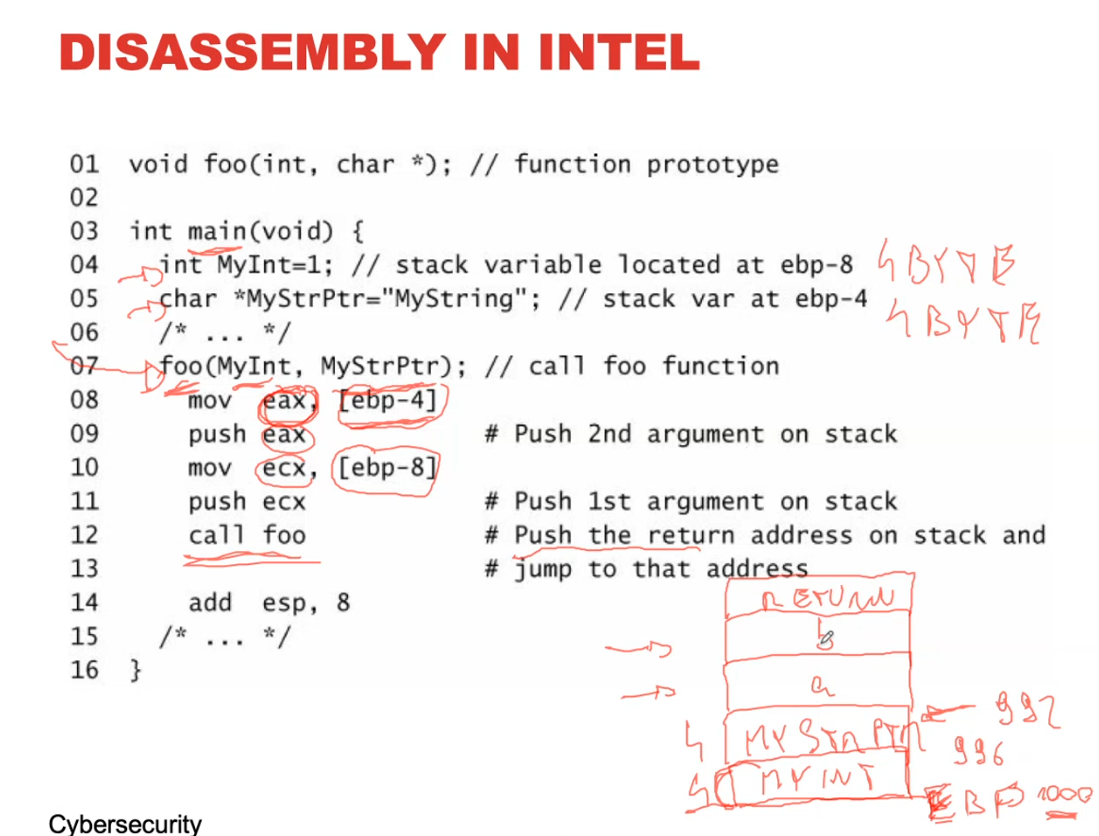
\includegraphics[width=13cm, keepaspectratio]{capitoli/secure_coding/img/cap_2/disass_intel_1.png}
    \caption{Esempio disassembly main in intel.}\label{fig:disass_intel_1}
\end{figure}

Vediamo ora come si comporta la funzione \verb|foo| quando viene chiamata, Figura \ref{fig:disass_intel_2}. Dopo aver salvato il return address salviamo anche l'ebp della funzione \verb|main| in modo da ricordarsi dove inizia il suo frame quando la chiamata di funzione \verb|foo| termina. Dopo ebp di main inizia il frame di \verb|foo| dove verranno salvate tutte le sue variabili locali, esso è grande 28 byte.
\begin{enumerate}
    \item \verb|push ebp|: salva il puntatore al frame corrente ovvero ebp di main;
    \item \verb|mov ebp, esp|: salviamo il puntatore alla fine del frame di main esp nel ebp, in modo da iniziare il frame di foo alla fine di quello del main;
    \item \verb|sub esp, 28|: allochiamo 28 byte di spazio per foo con esp - 28.
\end{enumerate}
\begin{figure}[H]
    \centering
    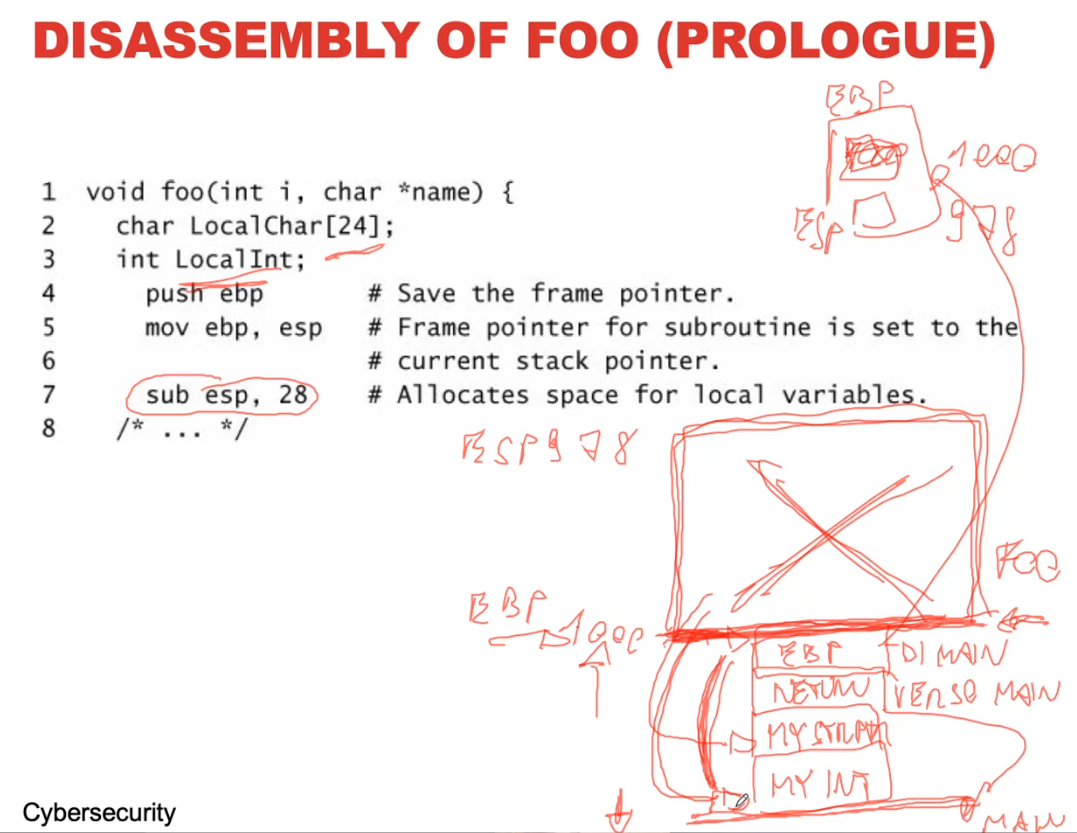
\includegraphics[width=13cm, keepaspectratio]{capitoli/secure_coding/img/cap_2/disass_intel_2.png}
    \caption{Esempio disassembly foo in intel.}\label{fig:disass_intel_2}
\end{figure}

Come si può vedere anche nell'immagine sottostante, il frame di foo è costituito dai seguenti elementi in questo ordine:
\begin{enumerate}
    \item Primo parametro della funzione foo: \verb|toMyString| (4 byte);
    \item Secondo argomento: \verb|MyInt| (4 byte);
    \item Return address del main (4 byte);
    \item Ebp del main (4 byte);
    \item Prima variabile locale \verb|LocalChar| (24 byte);
    \item Seconda variabile locale \verb|LocalInt|  (4 byte).
\end{enumerate}
\begin{figure}[H]
    \centering
    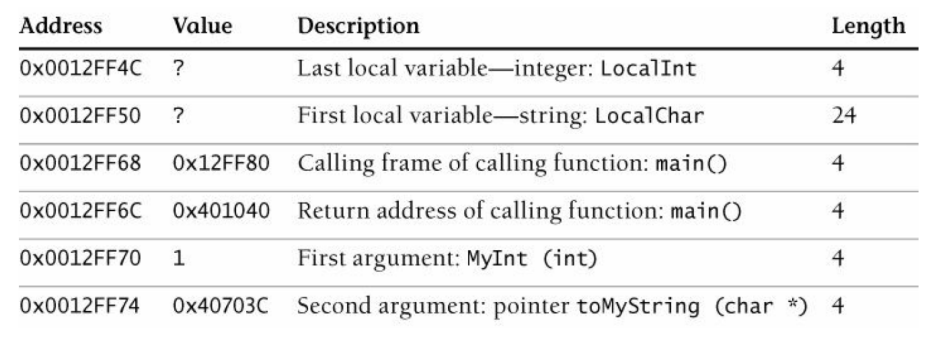
\includegraphics[width=13cm, keepaspectratio]{capitoli/secure_coding/img/cap_2/diss_stack.png}
    \caption{Frame di foo.}\label{fig:frame_foo}
\end{figure}
Infine vediamo cosa succede quando facciamo il return di foo, in generale lo scopo è di disallocare tutto lo spazio di memoria della funzione foo e di tornare all'istruzione successiva del main. Esso è composto da più comandi in assembly che sono:
\begin{enumerate}
    \item \verb|mov esp,ebp|: allo stack pointer esp inserisco il valore del ebp del frame corrente, ovvero si passa ad esempio da esp = 900 $\rightarrow$1000.
    \item \verb|pop ebp|: ristabilisce il frame pointer ebp con quello della funzione chiamante (main), ovvero disallocando i 28 byte del frame di foo il primo elemento che troviamo in memoria è proprio il valore del ebp del main che ci eravamo salvati in precedenza, facendo il pop lo eliminiamo dalla pila e lo reinseriamo nel registro della CPU;
    \item \verb|ret|: fa il pop del return address dallo stack, lo mette nel eip (prossima istruzione da fare ovvero tornare al punto di chiamata) e trasferisce il controllo a quel frame.
\end{enumerate}
Dopo aver fatto il return si esegue il prossimo comando che è appunto \verb|add esp, 8| in Figura \ref{fig:disass_intel_1}, il quale aggiunge all'esp 8 byte perché dalla memoria devono essere eliminati ancora i parametri passati alla funzione chiamata che sono MyStrPtr e MyInt. In questo modo si torna l'esp combacia con la parte alta del frame del main e l'ebp con l'inizio di quest'ultimo.
\begin{figure}[H]
    \centering
    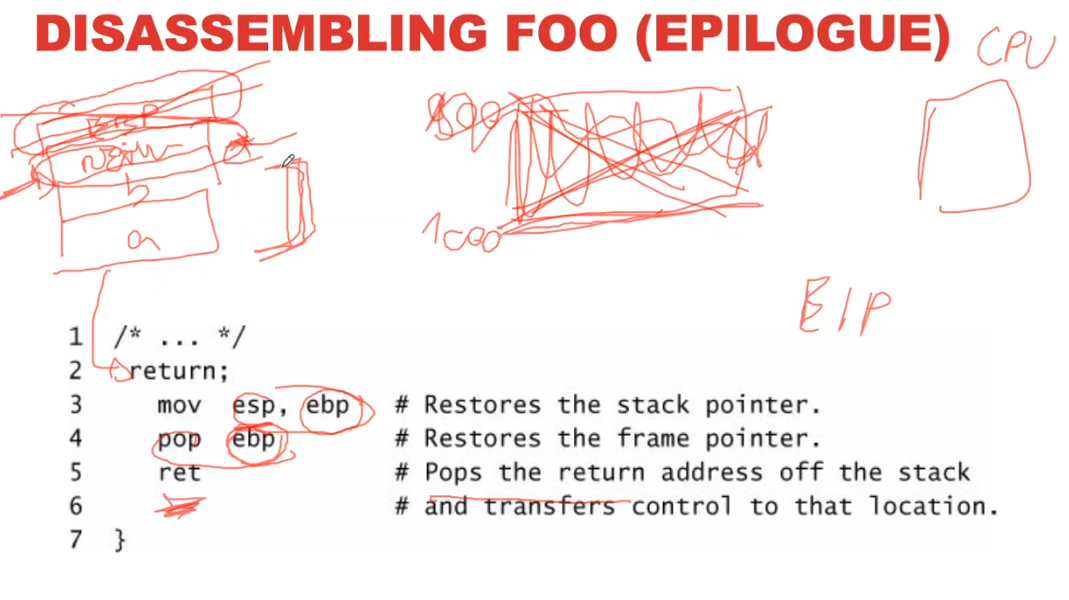
\includegraphics[width=13cm, keepaspectratio]{capitoli/secure_coding/img/cap_2/disass_intel_3.png}
    \caption{Return di foo.}\label{fig:disass_intel_3}
\end{figure}

\paragraph{Valori di ritorno.} Se ci sono dei valori di ritorno questi sono salvati in eax dalla funzione chiamata prima che ritorni al main. In questo modo la funzione chiamante sa dove si trovano i valori di ritorno e li può usare.
\begin{figure}[H]
    \centering
    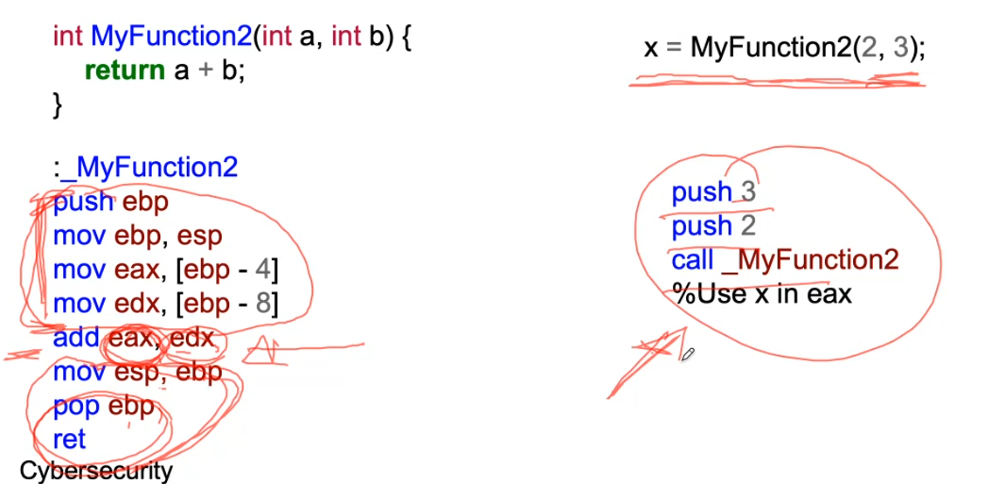
\includegraphics[width=13cm, keepaspectratio]{capitoli/secure_coding/img/cap_2/return_values.png}
    \caption{Valori di ritorno.}\label{fig:ret_values}
\end{figure}

\section{Stack smashing}
Stack smashing è quando un attaccante intenzionalmente fa overflow di un buffer nello stack per ottenere l'accesso a vietato regioni della memoria del computer. Questo avviene quando si riscrivono dei dati all'interno della memoria allocata all'esecuzione dello stack. Si possono avere delle serie conseguenze come ad esempio la modifica di valori delle \textbf{variabili automatiche} o l'esecuzione di codice arbitrario. Un esempio comune è sovrascrivere il return address che si trova nello stack.

\subsection{Arc Injection}
\subsubsection{Esempio \textit{IsPasswordOk}: Arc Injection} Nell'esempio in Figura \ref{fig:password} il programma è vulnerabile a stack smashing. Questo difetto può essere facilmente dimostrato inserendo una password di 20 caratteri  “1234567890123456 W$\triangleright$*!” che porta a far saltare il programma in modo imprevisto.
\begin{figure}[H]
    \centering
    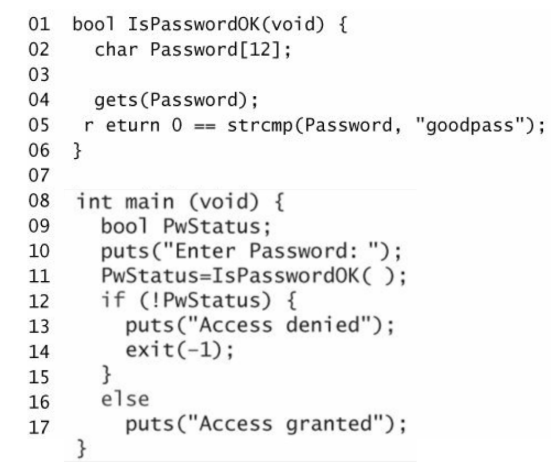
\includegraphics[width=8cm, keepaspectratio]{capitoli/secure_coding/img/cap_2/pass_ok_new.png}
    \caption{IsPasswordOk nuova.}\label{fig:pass_ok_new}
\end{figure}

\begin{figure}[H]
    \centering
    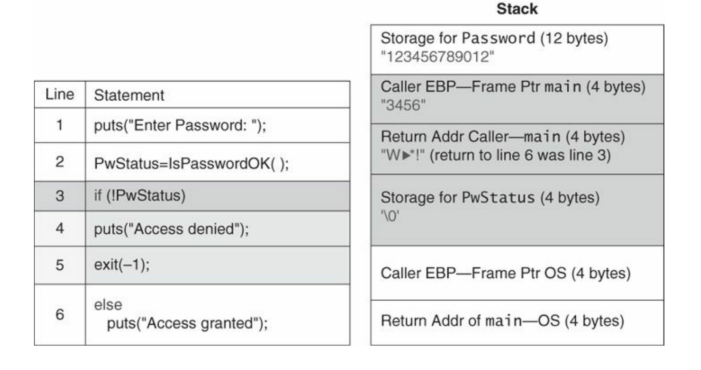
\includegraphics[width=13cm, keepaspectratio]{capitoli/secure_coding/img/cap_2/es_pass_ok_new.png}
    \caption{Funzionamento stack smashing.}\label{fig:es_pass_ok_new}
\end{figure}
In memoria l'ultima sequenza di quattro caratteri W$\triangleright$*! corrisponde a un indirizzo di 4 byte che sovrascrive l'indirizzo di ritorno nello stack, quindi invece di tornare all'istruzione subito dopo la chiamata in main() ritorna al ramo “Access granted” bypassando così il controllo della password e autorizzando ad avere accesso al sistema.
Un metodo per capire dove è salvato il return address di una funzione nello stack è l'utilizzo del comando
\verb|void * __builtin_return_address (unsigned int level)| il quale permette di con un valore di 0 di avere il return address della funzione corrente e con un valore di 1 ritorna il valore della funzione chiamante. Questa tecnica di buffer overflow si chiama \textbf{Arc Injection}.


La tecnica di \textbf{Arc Injection} (a volte chiamata \textbf{return into-libc}) prevede il trasferimento del controllo al codice esiste già nella memoria di processo.
Questi exploit sono chiamati così perché inseriscono un nuovo arco (trasferimento del flusso di controllo) nel flusso di controllo del programma invece di iniettare nuovo codice. Questa tecnica è preferita rispetto al code injection per vari motivi:
\begin{itemize}
    \item Si utilizza del codice che si trova già in memoria nel sistema preso di mira, in questo modo le \textbf{impronte lasciate dall'attaccante sono significativamente minori};
    \item Essendo che questo metodo si basa su codice esistente, n\textbf{on può essere bloccato da schemi di protezione basati sulla memoria} come la creazione di segmenti di memoria non eseguibile.
\end{itemize}

\subsection{Code Injection (Shell Code)}
Quando l'indirizzo di ritorno viene sovrascritto a causa di un software difetto, raramente indica istruzioni valide. Per un attaccante è possibile creare delle stringhe speciali che contengono \textbf{un puntatore a qualche codice malevolo}, sempre creato dall'attaccante. Questo implica che quando il return address sovrascritto viene invocato il controllo è trasferito al codice iniettato, il quale viene eseguito con i permessi del programma. Per questo i programmi che vengono eseguiti con permessi di \textbf{root} o dei \textbf{privilegi elevati} sono il target di certi attacchi, infatti frequentemente il codice malevolo apre una shell remota \textbf{(shellcode)} nella macchina compromessa permettendo all'attaccante di inserire dei comandi.

\subsubsection{Esempio \textit{IsPasswordOk}: Code Injection.} Prendendo sempre come esempio il programma "IsPasswordOk" \ref{fig:pass_ok_new}.

\begin{figure}[H]
    \centering
    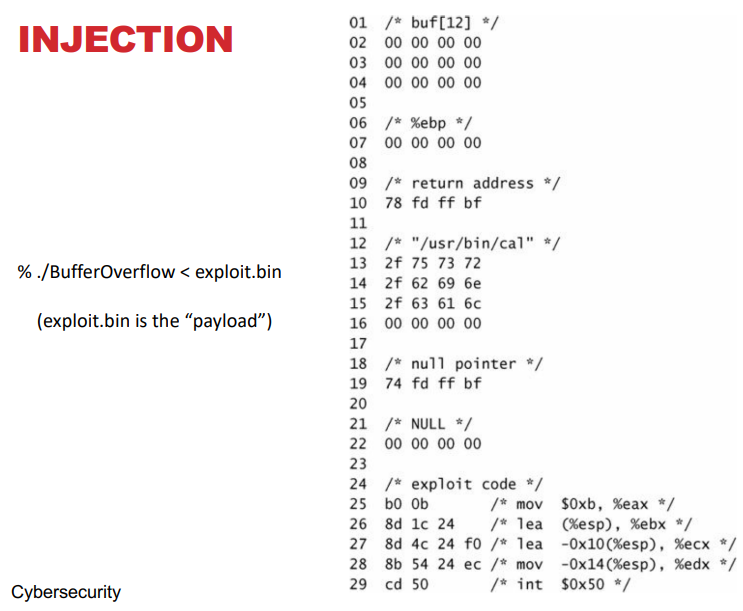
\includegraphics[width=12cm, keepaspectratio]{capitoli/secure_coding/img/cap_2/es_pass_ok_code_inj.png}
    \caption{Esempio con Code Injection}\label{fig:es_pass_ok_code_inj}
\end{figure}
Anche in questo caso cerchiamo di sovrascrivere il segmento del return address in modo da farlo puntare al nostro codice malevolo che possiamo vedere al commento "exploit code". Il nostro payload, ovvero il nostro codice, è tutto scritto in esadecimale per comodità invece che in binario. Partiamo inserendo 12 caratteri nella variabile "Password" successivamente sovrascriviamo il puntatore ebp con 4 interi causuali, non ci interessa questa zona. Arriviamo infine al punto che ci interessa ovvero il segmento del return address nel quale inseriremo come valore l'esadecimale del segmento dove salviamo il codice di exploit in modo da eseguirlo. Prima di eseguire quest'ultimo salviamo 3 parametri che passeremo successivamente alle funzioni del exploit:
\begin{itemize}
    \item \textbf{"/usr/bin/cal"}: il primo esadecimale si traduce con il comando \verb|/usr/bin/cal|.
    \item \textbf{"null pointer"}: il secondo è un puntatore a null.
    \item \textbf{"NULL"}: caratteri nulli.
\end{itemize}

\textbf{Spiegazione exploit code.} Vediamo nel dettaglio cosa fanno i comandi scritti in esadecimale del nostro exploit code.
\begin{itemize}
    \item \verb|mov $0xb, %eax|: assegna 0xB, il quale identifica il numero della chiamata di sistema \verb|execve()|, al registro \%eax; \\
          \verb|int execve(const char *filename, char *const argv[], char *const envp[]);|
    \item \verb|lea (%esp), %ebx|: "load effective address", calcola l'indirizzo effettivo del secondo operando (operando sorgente) e lo salva nel primo (operando destinatario). L'operando sorgente è un indirizzo di memoria (parte offset) specificato con una delle modalità di indirizzamento del processore mentre l'operando di destinazione è un registro di uso generale. In questo caso vengono inseriti i tre parametri, salvati in precedenza agli indirizzi (\%esp), -0x10(\%esp) (esp-16) e -0x14(\%esp)(esp-20), nei registri ebx, ecx ed edx.
          \item\verb|int 0x50|: chiamata vera e propria  per invocare execve(), che comporta l'esecuzione del programma di calendario Linux.
\end{itemize}
\begin{figure}[H]
    \centering
    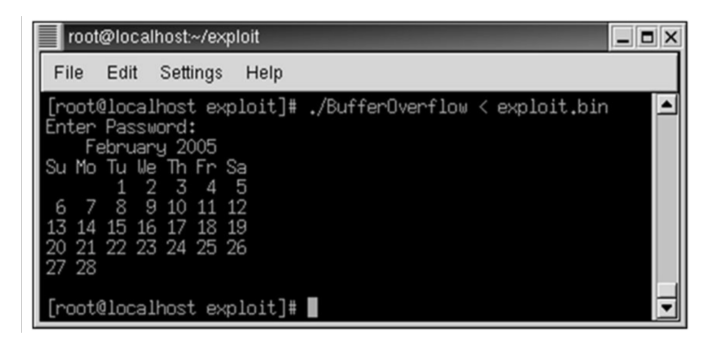
\includegraphics[width=12cm, keepaspectratio]{capitoli/secure_coding/img/cap_2/risultato_ex_pass_code_inj.png}
    \caption{Risultato esempio Code Injection.}\label{fig:ris_es_pass_ok_code_inj}
\end{figure}





    \chapter{Return-oriented Programming ROP}

ROP è una tipologia di attacco a basso livello, assembly.
Quando si compila un codice, viene caricata in quasi tutti i programmi Unix anche la
libreria standard \textbf{libc}, la quale contiene delle routine utili per un attaccante.
Per l'attacco vengono utilizzate solo piccole sequenze di codice, esse sono lunghe
solo due o tre istruzioni (\textbf{gadget}). Alcune di esse sono presenti in \textbf{libc}
come risultato delle scelte fatte dal compilatore durante la generazione del codice.

\section{Funzionamento dell'attacco}

La ROP è una tecnica simile all'Arc Injection, ma invece di ritornare alle funzioni,
il codice di exploit ritorna a sequenze di istruzioni seguite da un return (\textbf{ret}).
Ogni sequenza di istruzioni utile è chiamata \textbf{gadget},
ognuno di essi specifica determinati valori da inserire nello stack che permettono
di usare queste sequenza di istruzioni.
Essi sono delle istruzioni come load, add o jump. Questa tecnica permette all'attaccante
di eseguire codice in presenza di difese di sicurezza
come \textit{executable space protection}
\footnote{ Nella sicurezza del computer, la protezione dello spazio eseguibile contrassegna
    le regioni di memoria come non eseguibili,
    in modo tale che un tentativo di eseguire codice macchina in queste regioni causerà un'eccezione}
e \textit{code signing}
\footnote{La firma del codice è il processo di firma digitale di eseguibili e script
    per confermare l'autore del software e garantire che
    il codice non sia stato alterato o danneggiato da quando è stato firmato.}

\paragraph{Esempio gadget.} Il gadget che vediamo in questo esempio
è \verb|pop %ebx; ret;|, costituito da due istruzioni. A sinistra possiamo vedere
il suo corrispettivo nel linguaggio assembly il quale copia il valore
costante \verb|$0xdeadbeef| nel registro ebx e poi passa all'istruzione successiva
grazie al puntatore eip, mentre la parte destra mostra il gadget equivalente.

\begin{figure}[H]
    \centering
    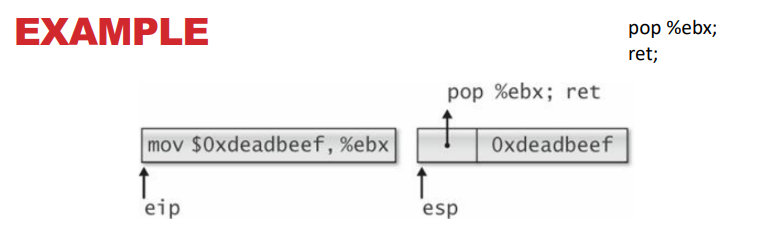
\includegraphics[width=13cm, keepaspectratio]{capitoli/secure_coding/img/cap_3/es_gadget.png}
    \caption{Esempio gadget.}\label{fig:es_gadget}
\end{figure}

Il gadget funziona nel seguente modo:

\begin{itemize}
    \item fa una pop del valore \verb|$0xdeadbeef| che si trova nello stack e lo
          inserisce nel registro ebx, facendo una pop viene diminuito anche la grandezza
          dello stack in base a quanto occupava quel valore in memoria. In questo caso si
          lavora con l'esp perché si tiene conto della fine del frame che diminuisce;
    \item infine fa una ret che permette di eseguire il gadget successivo nello stack,
          come eip. Il nostro scopo è di creare una catena di gadget, composizione di varie
          operazioni, per l'attacco.
\end{itemize}

\paragraph{Esempio di attacco.}
L'obiettivo dell'attacco è di invocare la chiamata di sistema \\
\verb|ssize_t sys_write(unsigned int fd, const char * buf, size_t count)|
in modo da stampare a schermo “xxxHACKEDxxx”. Questa istruzione prende in input
un \textit{file descriptor} in questo caso un stdout, una stringa e la dimensione
della stringa da stampare.

\begin{figure}[H]
    \centering
    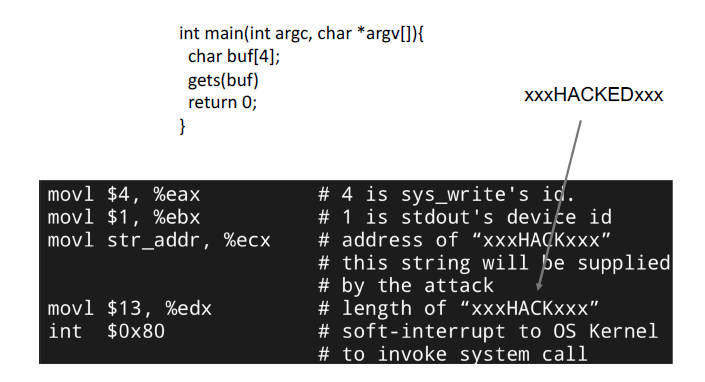
\includegraphics[width=13cm, keepaspectratio]{capitoli/secure_coding/img/cap_3/es_attacco_rop.png}
    \caption{Esempio attacco ROP.}\label{fig:es_attacco_rop}
\end{figure}

Vediamo nel dettaglio come funziona, per inserire il codice nello stack possiamo
fare un buffer overflow come abbiamo visto nell'esempio del code injection:

\begin{enumerate}
    \item \verb|movl $4, %eax|: inserisce
          l'identificatore della sys\_write nel registro eax;
    \item \verb|movl $1, %ebx|: inserisce l'identificatore
          dello standard output stdout nel registro ebx;
    \item \verb|movl str_addr, %ecx|: copia l'indirizzo della stringa nel registro ecx;
    \item \verb|movl $13, %edx|: inserisce la grandezza della
          stringa nel registro edx, in questo modo abbiamo caricato nella
          CPU tutto quello che ci serve. Per prima mette la chiamata di
          sistema sys\_write e poi tutti i suoi parametri che abbiamo visto in
          precedenza;
    \item \verb|int $0x80|: int interrompe l'esecuzione della CPU e salta al
          valore salvato in eax che è 4 ovvero la funzione sys\_write.
\end{enumerate}

Proviamo a fare lo stesso attacco con i gadget.

\begin{figure}[H]
    \centering
    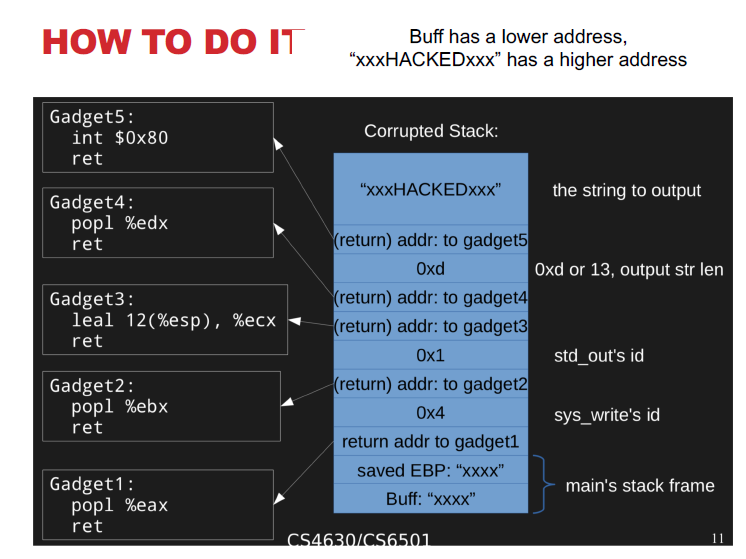
\includegraphics[width=13cm, keepaspectratio]{capitoli/secure_coding/img/cap_3/es_attacco_rop_gadget.png}
    \caption{Esempio attacco ROP con gadget.}\label{fig:es_attacco_rop_gadget}
\end{figure}

Nel caso di ROP, non c'è bisogno di scrivere un programma ma è necessario andare a
trovare, all'interno della \textbf{libc} ad esempio, dei gadget equivalenti alle
istruzioni viste in precedenza.
Come si può vedere in Figura \ref{fig:es_attacco_rop_gadget} partendo dal basso verso
l'alto dove il buff ha un indirizzo più basso rispetto
alla stringa “xxxHACKEDxxx”, abbiamo i primi due spazi di memoria dedicati al main
frame con l'ebp e il buffer,
successivamente la prima istruzione da effettuare è la \textbf{ret} del Gadget1.
La ret permette di eliminare tutto quello che ci stava prima di "0x4" compreso il
"return addr to gadget1" per poi passare a eseguire la prossima
istruzione del gadget1 che è \textbf{pop \%eax}.
Questa operazione è simile al funzionamento di eip ovvero esso contiene l'istruzione
successiva da eseguire senza eliminare quello che è salvato prima.
Facendo la pop si elimina a sua volta quello che sta contenuto nella porzione di
memoria successiva al return addr del gadget1 ovvero 0x4 e lo
inserisce nel registro eax. Si continua così per tutti gli altri gadget.
Nel Gadget3 si inserisce l'indirizzo di memoria della stringa che vogliamo stampare
che è \textbf{12(\%esp)}
ovvero 12 byte sotto rispetto all'esp, il quale punta dopo la ret all'inizio
di "return addr: to gadget 4".

\subsection{Qualche problema teorico}

In generale se il file eseguibile è più grande di 3 MB c'è una buona probabilità
che si può trovare un insieme di gadget per ogni exploit, più il file è piccolo più
diminuisce la probabilità di trovare dei gadget. Inoltre non è sempre necessario usare
la ret ma possiamo usare anche il jump o altre, i ROP possono lavorare anche
senza \textbf{libc} ma utilizzando il codice fornito. La tecnica ROP fornisce un
"linguaggio" (Turing complete) completamente funzionale che un utente malintenzionato
può utilizzare
in modo da far eseguire  qualsiasi operazione desiderata a una macchina compromessa.

\subsection{Come si fa exploit/previene}

Il tool \textit{ROPgadget} è uno strumento automatizzato per aiutare ad automatizzare
il processo di individuazione dei gadget e costruzione di un attacco contro un file
binario. Esso ricerca all'interno del file binario dei potenziali gadget utili e
tenta di assemblarli in un payload di attacco che produce una shell. Un altro modo
semplice di creare un attacco ROP è tramite il framework
CTF(Capture The Flag) \textbf{pwtools} \footnote{http://docs.pwntools.com/en/stable/rop/rop.html},
scritto in Python è stato progettato per la prototipazione rapida e per rendere
la scrittura di exploit il più semplice possibile.


\newpage
\section{Forme di mitigazione}

Nella versione 4.1, GCC ha introdotto \textbf{Stack-Smashing Protector (SSP)},
che implementa i canarini derivati da StackGuard.

\subsection{Stack-Smashing Protector}

SSP o ProPolice è un estensione di GCC per la protezione delle applicazioni scritte
in C dalle più comuni forme di exploit di buffer overflow. Esso riordina le variabili
locali in modo da mettere i buffer dopo i puntatori e copia i puntatori che si trovano
negli argomenti delle funzioni in un'area che precede i buffer delle variabili locali
in modo da evitare la corruzione dei puntatori.

\subsection{I canarini}

I canarini consistono in un valore difficile da inserire o falsificare e sono scritti
in un indirizzo prima della sezione della pila da proteggere.
Di conseguenza, una scrittura sequenziale dovrebbe sovrascrivere questo valore per
arrivare alla regione protetta.

\begin{figure}[H]
    \centering
    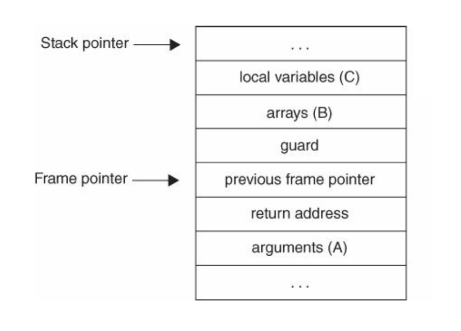
\includegraphics[width=12cm, keepaspectratio]{capitoli/secure_coding/img/cap_3/canarini.png}
    \caption{Canarino nello stack.}\label{fig:canarini}
\end{figure}

Come si può vedere in Figura \ref{fig:canarini}, il canarino viene inizializzato dopo
che il return address è salvato ed è verificato
immediatamente prima di accedere a quest'ultimo. Un canarino casuale o difficile da
falsificare è un numero casuale segreto a 32-bit che cambia ogni
volta che il programma viene eseguito. Le opzioni \verb|-fstack-protector|
e \verb|-fno-stack-protector| abilitano o disabilitano SSP per la protezione di
oggetti vulnerabili.

\subsection{Address Space Layout Randomization}

L' ASLR è una caratteristica della sicurezza di molti sistemi operativi, il suo scopo
è di evitare l'esecuzione di codice arbitrario. Essa permette di randomizzare gli
indirizzi delle pagine di memoria usate dal programma. Però ASLR non previene la
sovrascrittura del return address da parte di un overflow basato sullo stack. In ogni
caso esso potrebbe prevenire la predizione corretta da parte degli attaccanti
dell'indirizzo dello shellcode, delle funzioni di sistema dei gadget ROP che
vogliono invocare.

\subsection{Stack non-eseguibile}

Uno stack non eseguibile è una soluzione runtime (a tempo di esecuzione) che è stata
progettata per prevenire l'esecuzione di codice eseguibile  nel segmento dello stack.
Esso previene il buffer overflow solo sullo stack non sull'heap, inoltre non prevengono
il fatto di poter usare l'overflow per un modificare un indirizzo di ritorno, un
puntatore ad un oggetto o ad una funzione. Non prevengono la code o arc injection
o la ROP.

\subsection{W xor X}

Molti sistemi operativi, come OpenBDS, Windows, Linux e OS X, impone privilegi ridotti
nel kernel così
che nessuna parte dello spazio degli indirizzi del processo è sia scrivibile che
eseguibile.
Questa politica è chiamata W xor X (W$\bigoplus$X) ed è supportato dall'uso di un
bit No eXecute (NX) attivo in diverse CPU.
    \chapter{Heap Overflows}
\subsection{Alcuni problemi dello heap}
Il problema riguardante la heap memory occorre quando essa non viene adeguatamente liberata
dopo che non è più necessaria. Le memory leaks possono essere problematiche in processi a lungo termine
o in attacchi di esaurimento delle risorse. La memoria può essere \textbf{esausta} quando un malitenzionato identifica delle azioni esterne che possono allocare memoria ma non liberarla. Di conseguenza le allocazioni successive  falliscono e l'applicazione è incapace di processare delle richieste valide dello user senza \textbf{crashare}. Inoltre è possibile accedere alla memoria liberata a meno che tutti puntatori che puntano a quella memoria sono settati a NULL o sovrascritti. Perciò quando si libera, bisogna impostare anche il puntatore alla memoria liberata a NULL.

\paragraph{Dereferencing Null or Invalid Pointers.} Se l'operando non punta a un oggetto o una funzione, il comportamento dell'operatore unario * non è definito.

\paragraph{Double free.} Consiste nel liberare lo stesso blocco di memoria più di una volta.

\section{Heap overflow}
\subsection{Dlmalloc}
Nella dlmalloc, i blocchi di memoria (chunks) sono sia allocati a un processo che liberi. I primi 4 byte dei chunk allocati e liberi contengono la dimensione del precedente blocco adiacente, se è libero, ovvero gli ultimi 4 byte di dati utente del precedente pezzo, se è allocato.

\begin{figure}[H]
    \centering
    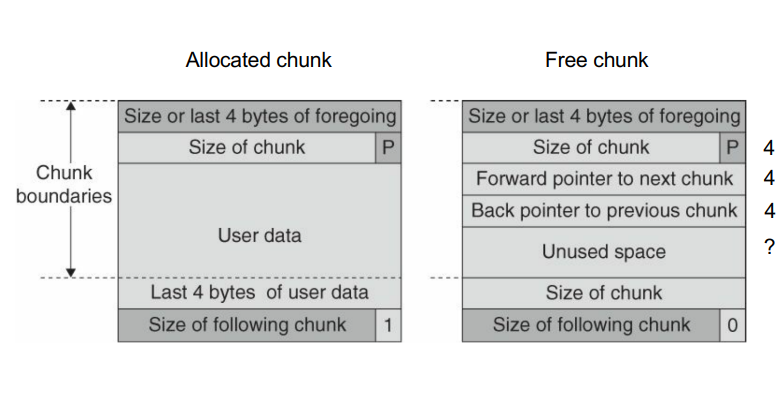
\includegraphics[width=13cm, keepaspectratio]{capitoli/secure_coding//img/cap_4/chuncks.png}
    \caption{Chunck libero e allocato.}\label{fig:chunck_lib_alloc}
\end{figure}

\subsubsection{Chunck liberi}
In dlmalloc, i blocchi liberi sono disposti in linked list
\footnote{In informatica, una lista concatenata (o linked list) è una struttura dati dinamica, tra quelle fondamentali usate nella programmazione.
    Consiste di una sequenza di nodi, ognuno contenente campi di dati arbitrari ed uno o due riferimenti ("link") che puntano al nodo successivo e/o
    precedente.}
circolari a doppio collegamento, detti anche \textbf{bin}.
Ogni linked list a doppio collegamento ha un'intestazione che contiene un puntatore in avanti e indietro rispettivamente al primo e all'ultimo blocco
nella lista. Sia il puntatore in avanti dell'ultimo chunck che quello all'indietro nel primo chunck della lista punta all'elemento testa.
Quando la lista è vuota, i puntatori della testa fanno riferimento alla testa stessa.

\subsubsection{Bin}
Ogni bin ha una \textit{head}(testa) che contiene il puntatore in avanti e indietro che puntano rispettivamente al primo e all'ultimo blocco nella lista. Sia il chunck allocato che quello libero fanno uso di un bit \verb|PREV_INUSE| (rappresentato da P \ref{fig:bin}) che indica se il chunck precedente è allocato o meno.

\begin{figure}[H]
    \centering
    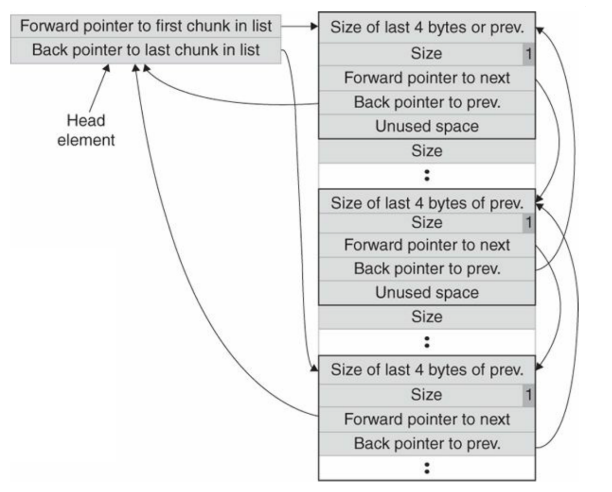
\includegraphics[width=12cm, keepaspectratio]{capitoli/secure_coding/img/cap_4/bin.png}
    \caption{Esempio di un bin.}\label{fig:bin}
\end{figure}
Sia il puntatore in avanti nell'ultimo chunck che quello indietro nel primo chunck della lista puntano alla testa. Quando la lista è vuota, la testa del puntatore si riferisce direttamente a se stessa.  Ogni
\subsubsection{UNLINK}
\verb|unlink()| è una macro usata per rimuovere un chunck dalla sua lista doppiamente linkata. Essa è usata quando la memoria è consolidata e quando un chunck è tolto della lista libera perchè è stato allocato da un utente.
\begin{verbatim}
    #define unlink(P, BK, FD) {
        FD = P -> fd;
        BK = P -> bk;
        FD -> bk = BK;
        BK -> fd = FD;
    }
\end{verbatim}

\paragraph{Funzionamento macro.}
Dalla Figura \ref{fig:ulink} si può capire bene il funzionamento della macro, essa prende in input tre puntatori
\begin{itemize}
    \item \textbf{P} puntatore al blocco da rimuovere;
    \item \textbf{BK} puntatore al blocco precedente;
    \item \textbf{FD} puntatore al blocco successivo.
\end{itemize}


\begin{figure}[H]
    \centering
    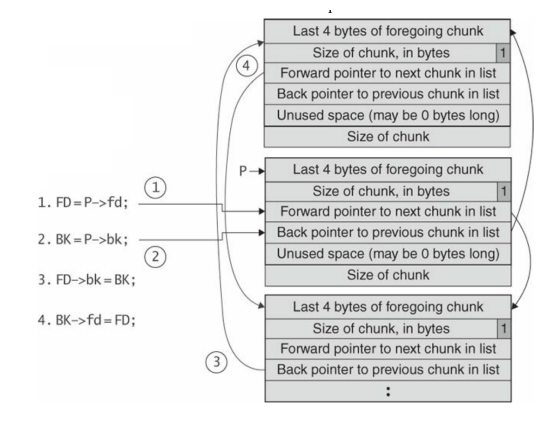
\includegraphics[width=12cm, keepaspectratio]{capitoli/secure_coding/img/cap_4/ulink.png}
    \caption{Funzionamente macro ulink.}\label{fig:ulink}
\end{figure}

In Figura \ref{fig:ulink} possiamo vedere un esempio del funzionamento della macro. Come accennato in precedenza il puntatore P si riferisce al chunck da togliere, esso contiene due puntatori uno che punta al blocco precedente e uno a quello successivo. Nel primo step della \verb|unlink()| si assegna FD in modo da farlo puntare al chunck successivo nella lista rispetto a quello indicato da P. Facciamo la stessa cosa nel secondo step solo che assegniamo a BK il puntatore al chunck precedente. Nel terzo step, il puntatore in avanti (FD)  sostituisce il puntatore all'indietro del blocco successivo nella lista con il puntatore al blocco che precede quello che è stato scollegato. Nell'ultimo step il puntatore all'indietro (BK) sostituisce il puntatore in avanti del precedente chunck nella lista con il puntatore al blocco successivo.

\subsection{Tecnica unlink}
La tecnica unlink è stata introdotta la prima volta da Solar Designer e usata con successo contro alcune versioni dei browser di Netscape, traceroute e slocate che utilizzavano dlmalloc. Questa tecnica è usata per fare un buffer overflow in modo da manipolare i tag di confine su un chunck di memoria per ingannare la macro \verb|unlink()| facendole scrivere 4 byte di dati in una zona arbitraria.

\begin{figure}[H]
    \centering
    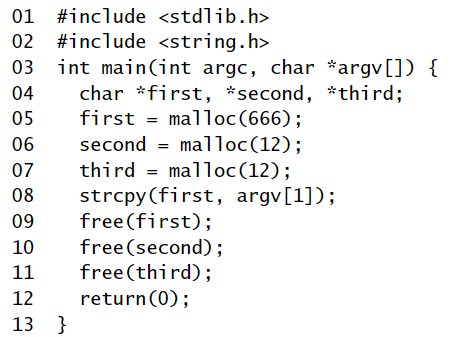
\includegraphics[width=10cm, keepaspectratio]{capitoli/secure_coding/img/cap_4/unlink_buff_over.png}
    \caption{Esempio di codice vulnerabile a tecnica unlink.}\label{fig:ulink_buff_over}
\end{figure}

Il programma vulnerabile alloca 3 chunck di memoria (riga 5-7). Il programma accetta una singola stringa come argomento che è copiata all'interno della malloc \textit{first} (linea 8). Questa operazione strcpy() illimitata è soggetta a un buffer overflow. Il tag di confine può essere sovrascritto da un argomento stringa che supera la lunghezza di first perché il tag di confine per il secondo si trova direttamente dopo il primo buffer. Il problema di questo programma accade alla seconda free (linea 10). Vediamo come è strutturato l'heap prima di fare la seconda free.

\begin{figure}[H]
    \centering
    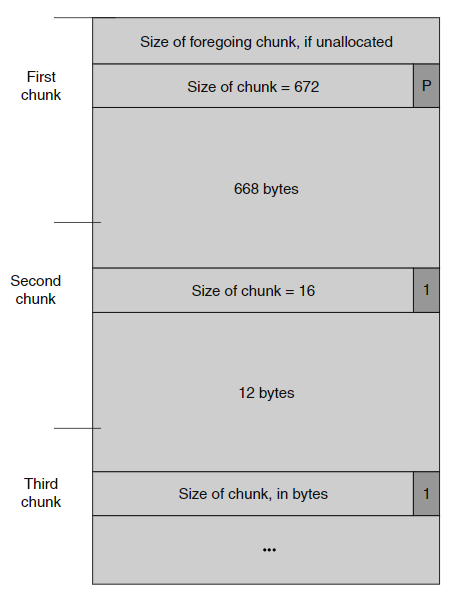
\includegraphics[width=10cm, keepaspectratio]{capitoli/secure_coding/img/cap_4/heap_prima_free.png}
    \caption{Contenuto dell'heap alla prima chiamata di free().}\label{fig:heap_prima_free}
\end{figure}
Se il secondo blocco non è allocato, l'operazione \verb|free()| prova a consolidarlo con il primo blocco. Per determinare se il secondo chunck è allocato o meno bisogna guardare il \verb|PREV_INUSE| bit del terzo blocco. La locazione di ogni blocco è determinata aggiungendo la grandezza del blocco all'indirizzo iniziale. Durante le operazioni normali, il bit P del terzo chunck è settato perchè il secondo chunck è allocato come si vede in Figura \ref{fig:heap_prima_free}.
Poiché il buffer vulnerabile è allocato nell'heap e non nello stack, l'attaccante non può solamente sovrascrivere l'indirizzo di ritorno per sfruttare la vulnerabilità ed eseguire codice malevolo. L'attaccante può sovrascrivere i boundary tag associati con il secondo chunck della memoria, perchè questo tag di confine è collocato immediatamente dopo la fine del primo blocco. La grandezza del primo chunck (672 byte) è il risultato della grandezza richiesta di 666 byte, più 4 byte per la grandezza, arrotondato al multiple più vicino a 8 poichè tutti chunck devono essere divisibili per 8 byte.
\begin{figure}[H]
    \centering
    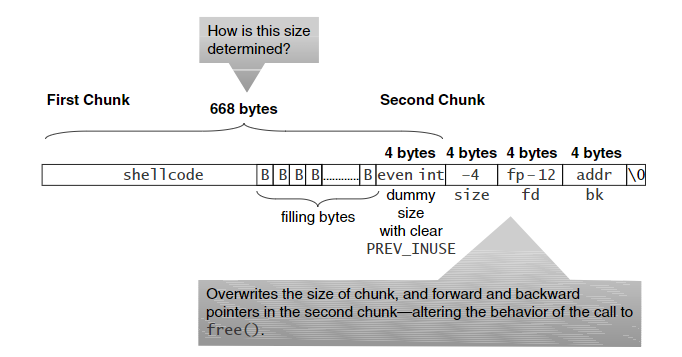
\includegraphics[width=13cm, keepaspectratio]{capitoli/secure_coding/img/cap_4/funzionamento_unlink.png}
    \caption{Funzionamento tecnica unlink.}\label{fig:funzionamento_unlink}
\end{figure}
Come si vede in Figura \ref{fig:funzionamento_unlink} un argomento malevolo può essere usato per sovrascrivere i tag del secondo chunck. Questo argomento sovrascrive il campo della dimensione del precedente blocco, grandezza del chunck, e i puntatori in avanti e indietro del secondo chunck, alterando così il comportamento della free(). In particolare il campo per la dimensione è modificato inserendo come valore -4 byte, in questo modo quando la free() prova a determinare la locazione del terzo chunck aggiungendo la grandezza appena modificata all'indirizzo iniziale del secondo chunck invece di aggiungere sottrae 4 byte. Così la dlmalloc pensa che l'inizio del successivo chunck è 4 byte prima dell'inizio del secondo chunck. L'argomento malevolo garantisce che la collocazione dove la dlmalloc trova il bit P è libera, ingannando la dlmalloc facendole credere che il secondo chunck non è allocato così l'operazione di free() invoca la unlink macro per consolidare i due blocchi liberi consecutivi. Come si vede in Figura \ref{fig:funzionamento_unlink} viene inserito al posto della grandezza effettiva del chunck un numero pari finto, deve essere pari poiché l'ultimo bit deve essere 0.  In fd inseriamo \verb|fp-12| che è l’indirizzo dove voglio compiere l’attacco. In bk c’è il dato che vogliamo scrivere all’indirizzo fd.
Per come è scritta la unlink, è lei stessa che fa questa cosa quando viene chiamata la seconda free.
Noi scriviamo solo il payload, poi il lavoro lo fanno free e di conseguenza unlink. L'obiettivo è scrivere l'indirizzo addr in fp.


    \chapter{Pointer subterfuge}

Il \textbf{pointer subterfuge} è un termine generale per gli exploit che modificano
il valore di un puntatore. In C e C++ esistono sia i puntatori a funzioni che i
puntatori a variabili.

\section{Puntatori a funzioni}

Nel caso dei puntatori a funzioni il valore di quest'ultimi può essere sovrascritto
in modo da trasferire il controllo a una shellcode fornita dall'attaccante.
Quando un programma esegue una  chiamata tramite il puntatore alla funzione, il codice
dell'attaccante è eseguito al posto del codice previsto.

\begin{figure}[H]
	\centering
	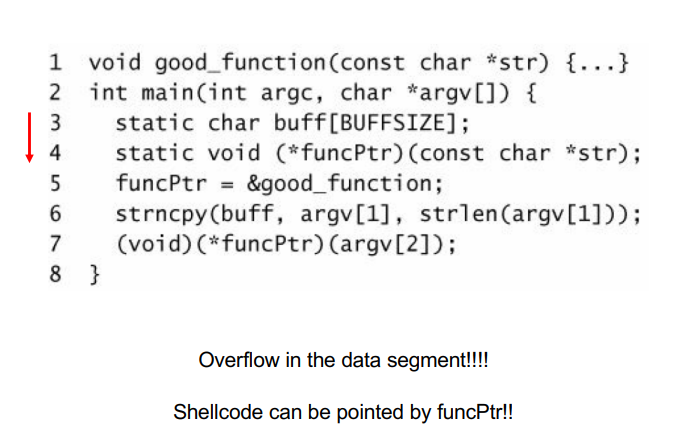
\includegraphics[width=10cm, keepaspectratio]{capitoli/secure_coding/img/cap_5/es_pointer_sub.png}
	\caption{Esempio pointer subterfuge su puntatori a funzioni.}\label{fig:es_poin_sub}
\end{figure}

Nel caso della Figura \ref{fig:es_poin_sub} il problema si trova nelle righe 3-4 poiché
non sappiamo la grandezza di \verb|BUFFSIZE| e questo può portare a un buffer overflow
sovrascrivendo il puntatore a funzione \verb|*funcPtr|. Abbiamo visto in precedenza
il buffer overflow applicato nello stack e nell'heap , in questo caso andiamo a
lavorare nella parte Data in cui vengono salvate le variabili sia globali che statiche.
Quindi le nostre variabili static \verb|buff[BUFFSIZE]| e \verb|*funcPtr| sono salvate,
presumibilmente una sotto l'altra, all'interno della parte Data della memoria.
In questo modo effettuando un buffer overflow si va a sovrascrivere il puntatore alla
funzione \verb|good_function| (riga 5), in seguito facendo uno \verb|strncpy| inserendo
più caratteri di quelli consentiti e richiamando la funzione tramite il suo
puntatore (riga 7) non si chiama effettivamente la \verb|good_function| ma
quello che abbiamo inserito noi.

\subsection{Puntatore a oggetti}

Lo stesso metodo può essere applicato ai puntatori a variabili.

\begin{figure}[H]
	\centering
	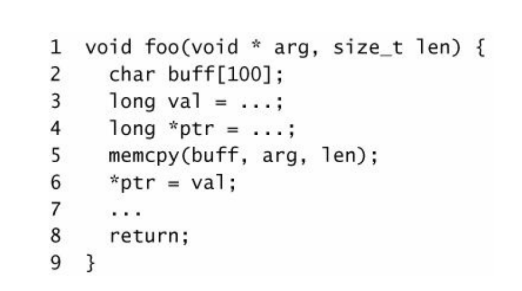
\includegraphics[width=10cm, keepaspectratio]{capitoli/secure_coding/img/cap_5/es_pointer_var.png}
	\caption{Esempio pointer subterfuge su puntatori a variabili.}\label{fig:es_poin_var}
\end{figure}

In questo caso abbiamo il \verb|buff[100]| di grandezza 100 caratteri seguito da
una variabile di tipo long e un puntatore sempre long. Nell'esempio di prima andavamo a
fare una \verb|strncpy| che portava al buffer overflow, qui invece facciamo
una \verb|memcpy(buff,arg,len)|\footnote{\textbf{void * memcpy ( void * destination,
		const void * source, size\_t num )}  Copia i valori dei byte di num, indica il numero di
	byte da copiare, dalla posizione a cui punta source direttamente nel blocco di memoria
	a cui punta destination.} che è sempre una copia non controllata da una zona sorgente
a una destinazione. Successivamente a riga 6 assegnando \verb|*ptr = val| scriviamo
un valore che vogliamo noi, poiché tramite il buffer overflow su buff[100] eccediamo
della grandezza massima e andiamo a sovrascrivere i valori delle successive variabili
a riga 3-4, in una zona di memoria che vogliamo noi quindi viene eseguita
una \textbf{scrittura di memoria arbitraria}.

\paragraph{Ultimo esempio}
Questo ultimo esempio differenzia da quelli precedenti per il modo in cui vengono
chiamate le funzioni, esse possono essere chiamate in modo diretto o indiretto.

\begin{figure}[H]
	\centering
	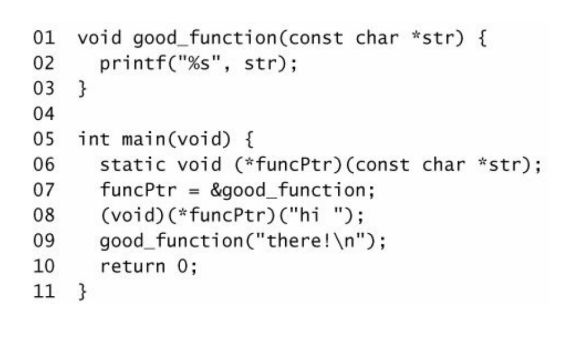
\includegraphics[width=10cm, keepaspectratio]{capitoli/secure_coding/img/cap_5/ult_es_point_sub.png}
	\caption{Esempio pointer subterfuge.}\label{fig:ult_es_poin}
\end{figure}

A riga 9 in Figura \ref{fig:ult_es_poin}possiamo vedere un esempio di chiamate diretta,
mentre a riga 8 abbiamo una indiretta poiché \verb|good_function| è chiamata tramite
il puntatore a quest'ultima. In Figura \ref{fig:dissas_ult_es_poin} vediamo a livello
assembly la differenza fra le due chiamate, la chiamate diretta è più semplice perché
viene effettuata, oltre la push per inserire nello stack la stringa da passare alla
funzione, direttamente una call a \textbf{good\_function}. Al contrario la chiamata
indiretta è un pò più complessa visto che non si fa una call
diretta a \textbf{good\_function} ma si chiama il puntatore a esse \verb|funcPtr|
che contiene l'indirizzo dove è salvata la funzione chiamata. L'istruzione di chiamata,
ad esempio, salva l'informazione di ritorno sullo stack e trasferisce il controllo
alla chiamata di funzione specificata dall'operando di destinazione (target). Il target
specifica l'indirizzo della prima istruzione nella funzione chiamata.

\begin{figure}[H]
	\centering
	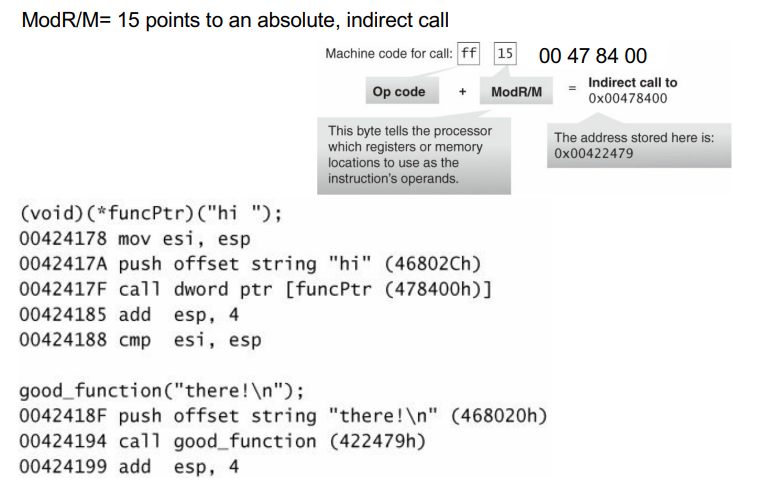
\includegraphics[width=12cm, keepaspectratio]{capitoli/secure_coding/img/cap_5/dissas_ult_es_point.png}
	\caption{Disassembly delle chiamate a \textbf{good\_function}.}\label{fig:dissas_ult_es_poin}
\end{figure}

Questo operando può essere un valore immediato, un registro generico, o una posizione
in memoria. Queste invocazioni di \textbf{good\_function()} forniscono esempi di
istruzioni di chiamata che possono e non possono essere attaccate. L'invocazione
statica utilizza un valore immediato come relativo spostamento, e questo spostamento
non può essere sovrascritto perché è nel segmento di codice. La chiamata tramite il
puntatore alla funzione utilizza un riferimento indiretto e l'indirizzo nella posizione
di riferimento può essere (in genere nel data o nel segmento dello stack) sovrascritto.

    \chapter{ID Managing}

\section{Intro}

Il \textbf{furto di identità} si verifica quando qualcuno utilizza le informazioni
personali di identificazione di un'altra persona, come il nome, il numero di
identificazione o il numero di carta di credito, senza il suo permesso,
per commettere frodi o altri crimini.

\subsection{Identità digitale}

Un'\textbf{identità digitale} è un'informazione su un'entità utilizzata dai sistemi
informatici per rappresentare un agente esterno.
Tale agente può essere una persona, un'organizzazione, un'applicazione o un
dispositivo.
\textit{ISO/IEC 24760-1} definisce l'\textbf{identità} come
"insieme di attributi relativi a un'entità".
Le informazioni contenute in un'\textbf{identità digitale} consentono di valutare
e autenticare un utente che interagisce con un sistema aziendale sul web/Network,
senza il coinvolgimento di operatori umani.

\subsection{Autenticazione}

L'autenticazione è un aspetto fondamentale nella verifica dell'identità
di tipo \textbf{trust-based}, che consiste nel fornire un'assicurazione
dell'identità codificata tra un'identità e l'altra.
Le \textbf{metodologie di autenticazione} includono la presentazione di
un \textbf{oggetto univoco} come una carta di credito bancaria,
le \textbf{informazioni riservate} come una una password o la risposta a una
domanda prestabilita, \textbf{la conferma della proprietà di un indirizzo e-mail}.
Le soluzioni più robuste ma relativamente costose utilizzando metodologie di
crittografia.

\subsection{Autorizzazione}

L'autorizzazione è l'atto di controllare che un'entità abbia diritto ad
accedere ed utilizzare determinate risorse, essa
dipende dall'autenticazione, perché l'autorizzazione richiede
la verifica dell'attributo critico.

\section{Identity}

I concetti di \textbf{identità}, \textbf{identificatore} e \textbf{account} sono
strettamente correlati ma diversi.

\subsection{Identifier}

Il termine "\textbf{identificatore}" si riferisce a un singolo attributo il cui scopo
è quello di identificare in modo univoco una persona o un'entità,
all'interno di un contesto specifico. Alcuni esempi sono
indirizzo email, numero passaporto, ecc... .

\subsection{Identità}

Il termine "identità" è definito come un insieme di attributi associati a una
specifica persona/entità in un particolare contesto. Un'identità comprende uno o
più identificatori e può contenere altri attributi associati a una persona/entità.

\subsubsection{Attributi}

Le identità umane possono includere attributi come il nome, età, indirizzo,
numero di telefono, colore degli occhi e titolo di lavoro.
Le identità non umane possono includere attributi come il proprietario,
l'indirizzo IP e forse un numero di modello o di versione.
Gli attributi che compongono un'identità possono essere utilizzati per
l'autenticazione e l'autorizzazione, oltre che per trasmettere informazioni
sull'identità alle applicazioni.
Un'identità online consiste in almeno un identificatore e un insieme di attributi
per un utente/entità in un particolare contesto, come un'applicazione o una suite di
applicazioni.

\subsection{Account}

Un'identità è associata a un account in ciascuno di questi contesti.
Definiamo un account come un costrutto locale all'interno di una data
applicazione o suite di applicazioni che viene utilizzato per eseguire azioni
all'interno di quel contesto.
Gli attributi di identità possono essere contenuti in una struttura chiamata
account object all'interno di un'applicazione,
oppure possono essere memorizzati separatamente e referenziati dall'account object.

\subsection{Separazione tra ID e Account}

Un account può avere un proprio identificativo oltre a quello dell'identità ad
esso associata. Avere un identificatore dell'account separato dall'identità
associata all'account fornisce un grado di separazione.
L'identificativo dell'account può essere utilizzato in altri record dell'applicazione
per rendere più facile per gli utenti cambiare il nome utente o altro identificatore
associato al proprio account.
Si noti che un account può avere più di un'identità associata ad esso attraverso
l'account linking.

\subsection{Non Human Identifier}

Anche gli attori non umani possono certamente avere un'identità.
I componenti software che fungono da agenti o bot e i dispositivi intelligenti
possono avere un'identità e possono interagire con altri software o dispositivi
in modi che richiedono autenticazione e autorizzazione, proprio come gli attori
umani.

\subsection{IDM System}

Un Identity Management System(IdM) è un insieme di servizi che supportano
la creazione, la modifica e la rimozione delle identità e degli account associati
ad esse,
nonché l'autenticazione e l'autorizzazione necessarie per accedere alle risorse.
I sistemi di gestione dell'identità sono utilizzati per proteggere risorse online
da accessi non autorizzati e costituiscono un parte importante di un modello di
sicurezza completo.

\section{Eventi in un ciclo di vita di un'identità}

\begin{figure}[H]
    \centering
    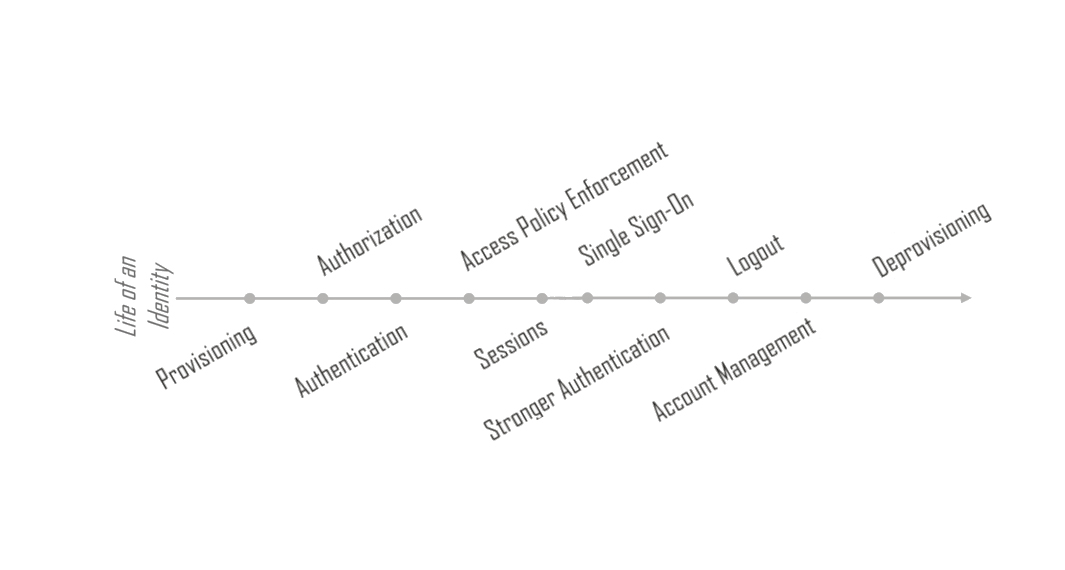
\includegraphics[width=\textwidth, keepaspectratio]{capitoli/id_managing/imgs/idman1.jpg}
\end{figure}

\subsection{PROVISIONING}

L'atto di creare un account e le relative informazioni di identità è spesso
indicato come provisioning.
L'obiettivo della fase di provisioning è quello di stabilire un account con i
relativi dati di identità.
Si tratta di ottenere o assegnare un identificativo univoco per l'identità,
opzionalmente un identificativo univoco per l'account distinto da quello
dell'identità, creare un account e associare gli attributi del profilo
dell'identità all'account.

\subsection{AUTHORIZATION}

Quando si crea un account, spesso è necessario specificare cosa può fare l'account,
sotto forma di privilegi.
Il termine autorizzazione indica la concessione di privilegi che regolano le attività
di un account.
L'autorizzazione di un account viene generalmente effettuata al momento della sua
creazione e può essere aggiornata nel tempo.

\subsection{AUTHENTICATION}

L'utente fornisce un identificativo per indicare l'account che desidera utilizzare e
inserisce le credenziali di accesso per l'account.
Queste vengono convalidate rispetto alle credenziali precedentemente registrate
durante la fase di provisioning dell'account.
Le credenziali possono riguardare qualcosa che l'utente conosce, qualcosa che
l'utente possiede e/o qualcosa che l'utente è.
Il nome utente indica l'account che l'utente desidera utilizzare e la conoscenza
della password dimostra il suo diritto a utilizzare l'account.

\subsection{ACCESS POLICY ENFORCEMENT}

%%TODO: ricontrollare tutto
L'autorizzazione specifica ciò che un utente o un'entità può fare. L'applicazione
dei criteri di accesso verifica che le azioni richieste da un utente siano
consentite dai privilegi che è stato autorizzato a utilizzare.

\subsection{SESSIONS}

Alcune applicazioni, in genere le applicazioni Web tradizionali e le applicazioni
sensibili, consentono a un utente di rimanere attivo solo per un periodo di tempo
limitato prima di richiedere all'utente di autenticarsi nuovamente.
(Una sessione tiene traccia delle informazioni)
Le impostazioni di timeout della sessione variano in genere in base alla
sensibilità dei dati dell'applicazione.

\subsection{SINGLE SIGN-ON}

Dopo aver effettuato l'accesso a un'applicazione, l'utente potrebbe voler
effettuare un'altra operazione con un'altra applicazione.
Il single sign-on (SSO) è la possibilità di effettuare il login una volta e poi
accedere ad altre risorse o applicazioni protette con gli stessi requisiti di
autenticazione, senza dover reinserire le credenziali.
Il single sign-on è possibile quando un insieme di applicazioni ha delegato
l'autenticazione alla stessa entità.

\subsection{STRONGER AUTHENTICATION}

L'autenticazione step-up è l'atto di elevare una sessione di autenticazione
esistente a un livello di garanzia più elevato mediante
autenticazione con una forma di autenticazione più forte.
Ad esempio, un utente potrebbe inizialmente accedere con un nome utente e una
password per stabilire una sessione di autenticazione.
In seguito, quando accede a una funzione o a un'applicazione più sensibile
con requisiti di autenticazione più elevati, all'utente vengono richieste
ulteriori credenziali, ad esempio una password una tantum generata sul suo
telefono cellulare.

\subsection{LOGOUT}

Come minimo, l'atto di disconnettersi dovrebbe terminare la sessione
dell'applicazione dell'utente.
Se l'utente ritorna all'applicazione, dovrà autenticarsi nuovamente prima di
poter accedere.
In situazioni in cui si utilizza il single sign-on, potrebbero esserci più
sessioni da terminare.
È una decisione di progettazione decidere quali sessioni debbano essere
terminare quando l'utente esce da un'applicazione.

\subsection{ACCOUNT MANAGEMENT AND RECOVERY}

Nel corso della vita di un'identità, può essere necessario modificare vari
attributi del profilo utente dell'identità.
Ad esempio, un utente potrebbe dover aggiornare il proprio indirizzo e-mail o
numero di telefono, la password e il nome.
In un'azienda, il profilo di un utente può essere aggiornato per riflettere una
nuova posizione, un nuovo indirizzo o nuovi privilegi come i ruoli.
Il recupero dell'account è un meccanismo per convalidare che un utente sia il
legittimo proprietario di un account attraverso alcuni mezzi secondari e quindi
consentire all'utente di stabilire nuove credenziali.
Ripristino della password smarrita via e-mail

\subsection{DEPROVISIONING}

Può capitare che sia necessario chiudere un account.
In questo caso, l'account dell'utente e le informazioni di identità associate
devono essere rimosse in modo che non possano più essere utilizzate.
Il deprovisioning può consistere nell'eliminazione completa dell'account e delle
informazioni di identità associate o nella semplice disabilitazione dell'account,
per conservare le informazioni a fini di revisione.
    % ...
    % Parte Bistarelli
    \part{Appunti parte Prof.Bistarelli}
    \chapter{ Cybersecurity }

\section{Introduzione alla sicurezza informatica}
Il rapporto interno/interagenzia NIST NISTIR 7298 (Glossario di informazioni chiave
Termini di sicurezza, maggio 2013) definisce il termine sicurezza informatica  come segue:

\begin{center}
    \textit{Misure e controlli che garantiscono riservatezza, integrità,
    e disponibilità delle risorse del sistema informativo inclusi hardware, software, firmware,
    e le informazioni che vengono elaborate, archiviate e comunicate.}
\end{center}


Questa definizione introduce tre obiettivi chiave che sono al centro della cybersecurity:

\begin{itemize}
    \item \textbf{Confidentiality} (Riservatezza):  conservazione delle restrizioni autorizzate all'accesso alle informazioni e divulgazione, compresi i mezzi per proteggere la privacy personale e le proprie informazione. Una perdita di riservatezza è la divulgazione non autorizzata di informazioni. Questo termine copre due concetti correlati:
    \begin{itemize}
        \item  \textbf{Data Confidentiality} : garantisce che le informazioni private o riservate non siano disponibili o divulgate a soggetti non autorizzati.
        \item \textbf{Privacy}: assicura che le persone controllino o influenzino le informazioni
        ad essi relativi, esse possono essere raccolte e conservate, inoltre si definisce da chi e a chi possono essere divulgate.
    \end{itemize}
    \item \textbf{Integrity} (Integrità): prevenire la modifica o la distruzione impropria delle informazioni, compresa la garanzia del non ripudio e dell'autenticità delle informazioni. Una perdita di l'integrità è la modifica o la distruzione non autorizzata di informazioni. Questo termine copre due concetti correlati:
    \begin{itemize}
        \item \textbf{Data integrity}:  garantisce che le informazioni e i programmi vengano modificati solo in modo determinato e autorizzato.
        \item \textbf{System integrity}: assicura che un sistema svolga la sua funzione prevista in modo inalterato, libero da intenzionali o involontarie manipolazioni non autorizzate del sistema.
    \end{itemize}
    \item \textbf{Availability}(Disponibilità): garantisce un accesso tempestivo e affidabile nell'utilizzo delle informazioni. Una perdita di disponibilità è l'interruzione dell'accesso o dell'uso di informazioni o un sistema informativo.
\end{itemize} 

\noindent
Questi tre concetti formano quella che viene spesso definita la triade della CIA. I tre
concetti incarnano gli obiettivi di sicurezza fondamentali sia per i dati che per le informazioni
e servizi informatici. Ad esempio, lo standard FIPS 199 del NIST (Standards for Security
Categorization of Federal Information and Information Systems , febbraio 2004) elenca la riservatezza, integrità e disponibilità come i tre obiettivi di sicurezza per le informazioni e
per i sistemi informativi.
\begin{figure}[H]
	\centering
    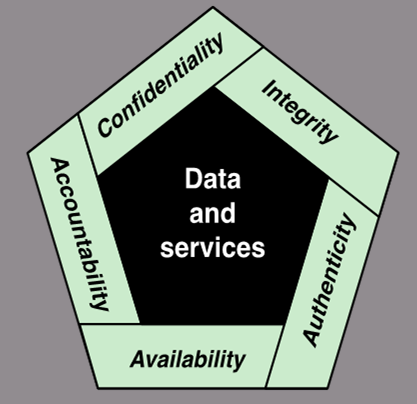
\includegraphics[width=7cm, keepaspectratio]{bistarelli/img/cap_1/cia.png}
	\caption{Requisiti essenziali in Cybersecurity.}\label{fig:cia}
\end{figure}

Sebbene l'uso della triade della CIA per definire gli obiettivi di sicurezza sia ben consolidato,
alcuni nel campo della sicurezza ritengono che siano necessari concetti aggiuntivi da presentare
un quadro completo. Due dei più comunemente citati sono i seguenti:
\begin{itemize}
    \item \textbf{Authenticity} (Autenticità): la proprietà di essere genuini e di poter essere verificati e di essere trusted. Fiducia nella validità di una trasmissione di un messaggio o di un messaggio originatore. Ciò significa verificare che gli utenti siano chi dicono di essere e che ogni input che arriva al sistema proviene da una fonte attendibile.
    \item \textbf{Accountability}(Rendicontabilità): è la capacità di un sistema di identificare un singolo utente, di determinarne le azioni e il comportamento all'interno del sistema stesso. La rendicontabilità è un aspetto del controllo di accesso e si basa sulla concezione che gli individui siano responsabili delle loro azioni all'interno del sistema. Questo supporta il non ripudio, deterrenza, isolamento dei guasti, rilevamento e prevenzione delle intrusioni, il recupero post-azione in concomitanza con l'azione legale . Poiché i sistemi veramente sicuri non sono ancora un obiettivo realizzabile, dobbiamo essere in grado di tracciare una violazione della sicurezza al/ai responsabile/i. I sistemi devono tenere traccia delle loro attività per consentire successive analisi forensi per rintracciare violazioni della sicurezza o per aiutare nelle controversie sulle transazioni.
\end{itemize}
Si noti che FIPS 199 include l'autenticità sotto integrità.
\\
La sicurezza informatica è allo stesso tempo affascinante e complessa, alcuni dei motivi sono:
\begin{enumerate}
    \item \textit{La sicurezza informatica non è così semplice come potrebbe sembrare a un principiante}. I requisiti sembrano essere semplici,in effetti, la maggior parte dei requisiti principali per i servizi di sicurezza possono essere definiti con etichette formate autoesplicative formate da una sola parola: riservatezza, autenticazione, non ripudio e integrità. Ma i meccanismi utilizzati per soddisfare tali requisiti possono essere piuttosto complessi, e capirli può portare a un ragionamento piuttosto sottile.
    \item \textit{Nello sviluppo di un particolare meccanismo di sicurezza o algoritmo, bisogna sempre considerare potenziali attacchi a tali funzionalità di sicurezza.} In molti casi gli attacchi di successo sono progettati guardando un problema in un modo completamente differente, dunque sfruttando una debolezza inaspettata del meccanismo.
    \item \textit{A causa del punto 2 , le procedure usate per fornire dei servizi particolari sono spesso controintuitive.} Tipicamente, un meccanismo di sicurezza è complesso e non è ovvio dalle dichiarazioni di una particolare esigenza che tali misure elaborate sono necessarie. Solo quando si prendono in considerazione i vari aspetti della minaccia si elaborano i meccanismi di sicurezza hanno un senso.
    \item \textit{I meccanismi di sicurezza in genere coinvolgono più di un particolare algoritmo o
    protocollo.}Richiedono inoltre che i partecipanti siano in possesso di un'informazione segreta (ad es. una chiave di crittografia), che sollevano domande sulla creazione, distribuzione e protezione di tali informazioni segrete. Potrebbe esserci anche una dipendenza sui protocolli di comunicazione il cui comportamento può complicare il compito di sviluppare il meccanismo di sicurezza. Ad esempio, se il corretto funzionamento del meccanismo di sicurezza richiede la definizione di limiti di tempo per il tempo di transito di un messaggio dal mittente al destinatario, allora qualsiasi protocollo o rete che introduce variabili e/o ritardi imprevedibili può rendere tali termini privi di significato.
    \item \textit{ La sicurezza informatica è essenzialmente una battaglia di ingegni tra un perpetratore che prova a  trovare buchi e il progettista o l'amministratore che tenta di chiuderli.} Il grande vantaggio che l'attaccante ha è che lei o lui ha solo bisogno di trovare una singola vulnerabilità, mentre il progettista deve trovare e eliminare tutte le vulnerabilità per ottenere una sicurezza perfetta.
    \item \textit{La sicurezza è ancora troppo spesso un'"aggiunta" (surplus) per essere incorporata in un sistema dopo che il progetto è completo, piuttosto che essere parte integrante del processo di progettazione.}
    \item \textit{La sicurezza richiede un monitoraggio regolare, anche costante, e questo è difficile nei tempi attuali.}
    \item \textit{C'è una naturale tendenza da parte di utenti e gestori di sistema a percepire pochi vantaggi nell'investimento sulla sicurezza fino a quando non si verifica un problema.}
    \item \textit{ Molti utenti e persino gli amministratori della sicurezza vedono una sicurezza forte come un ostacolo al funzionamento o all'uso efficiente di un sistema informativo o di un'informazione.}
\end{enumerate}

\subsection{Terminologie}
La maggior parte delle terminologie sono riportate nel Capitolo \ref{ch:terminologie} degli appunti Prof. Santini, di seguito riporto alcuni termini non citati in precedenza.

\subsubsection{Risorsa di sistema (Asset)}
Una applicazione maggiore, un sistema di supporto generale, un programma ad alto impatto,un impianto fisico, un sistema mission-critical, personale, apparecchiature o un gruppo di sistemi logicamente correlati.  

\subsubsection{Minaccia}
Qualsiasi circostanza o evento che potrebbe avere un impatto negativo sulle operazioni organizzative (inclusi missione, funzioni, immagine o reputazione), risorse organizzative, individui, altre organizzazioni o la Nazione stessa attraverso un sistema informativo tramite accesso, distruzione, divulgazione, modifica non autorizzati delle informazioni , e/o negazione del servizio.

\subsubsection{Contromisure}
Dispositivo o tecniche che hanno come obiettivo la compromissione dell'efficacia operativa di attività indesiderate o contraddittorie, o la prevenzione di spionaggio, sabotaggio, furto o accesso o utilizzo non autorizzato di informazioni sensibili o di sistemi informativi.

\subsubsection{Rischio}
Una misura del grado in cui un'entità è minacciata da una potenziale circostanza o evento, e tipicamente una funzione di stima:
\begin{enumerate}
    \item  degli impatti negativi che si verificherebbero se la circostanza o l'evento si verificassero
    \item  della probabilità che si verifichi.
\end{enumerate}

\begin{figure}[H]
	\centering
    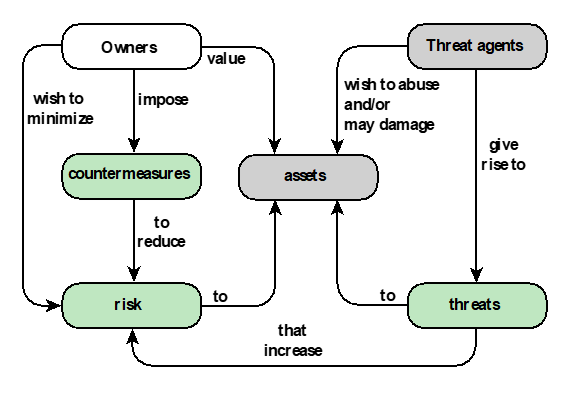
\includegraphics[width=11cm, keepaspectratio]{bistarelli/img/cap_1/relazione_concetti_sicurezza.png}
	\caption{Concetti di sicurezza e le loro relazioni.}\label{fig:relazioni_concetti_sec}
\end{figure}

\subsection{Asset di un sistema informatico}
Gli asset di un sistema informatico possono essere suddivisi come di seguito:
\begin{itemize}
    \item \textbf{Hardware}: compresi i sistemi informatici e altri trattamenti di dati, archiviazione dei dati,e dispositivi di comunicazione dati;
    \item \textbf{Software}: include il sistema operativo, le utilità di sistema e le applicazioni;
    \item \textbf{Data}: inclusi file e database, nonché dati relativi alla sicurezza, ad esempio file di password. 
    \item \textbf{Strutture e reti di comunicazione}: rete locale e geografica collegamenti di comunicazione, bridge, router e così via.
\end{itemize}

\subsection{Vulnerabilità, minacce e attacchi}
Nel contesto della sicurezza, la nostra preoccupazione riguarda le vulnerabilità delle risorse del sistema. [NRC02] elenca le seguenti categorie generali di vulnerabilità di un sistema informatico o di una risorsa di rete:
\begin{itemize}
    \item Il sistema può essere danneggiato (\textbf{corrupted}), quindi fa la cosa sbagliata o dà risposte sbagliate. Ad esempio, i valori dei dati memorizzati possono differire da quello che dovrebbero essere perché sono stati modificati in modo improprio.
    \item Il sistema avere delle perdite (\textbf{be leaky}). Ad esempio, qualcuno che non dovrebbe avere accesso ad alcune o a tutte le informazioni disponibili attraverso la rete ottengono tale accesso.
    \item Il sistema può diventare non disponibile (\textbf{unavailable}) o molto lento. Cioè, usando il sistema o la rete diventa impossibile o impraticabile.
\end{itemize}
Questi tre tipi generali di vulnerabilità corrispondono ai concetti di integrità, riservatezza e disponibilità, enumerati in precedenza. Una \textbf{minaccia} rappresenta un potenziale danno alla sicurezza di una risorsa. Un \textbf{attacco} è una minaccia che viene eseguita (azione di minaccia) e, in caso di successo, comporta una violazione indesiderata della sicurezza o a una conseguenza della minaccia. L'agente che effettua l'attacco viene definito \textbf{attaccante} o \textbf{agente di minaccia}. Possiamo distinguere gli attacchi in due tipi:
\begin{itemize}
    \item \textbf{Attacco attivo}: un tentativo di alterare le risorse del sistema o di influenzare il funzionamento.
    \item \textbf{Attacco passivo}: un tentativo di imparare o di fare use delle informazioni da un sistema che non influenza le risorse di quest'ultimo.
\end{itemize}

\noindent
Possiamo classificare gli attacchi in base all'origine di questi:
\begin{itemize}
    \item \textbf{Attacco interno}: iniziato da un entità interna al perimetro di sicurezza ( un "insider"). L'insider è autorizzato all'accesso alle risorse del sistema ma le usa in un modo non approvato da coloro che ne garantiscono l'accesso.  
    \item \textbf{Attacco esterno}: iniziato fuori dal perimetro, da un utente non autorizzato o illegittimo del sistema (un "outsider"). Su Internet, potenziale aggressori esterni variano dai dilettanti "burloni" a criminali organizzati, internazionali terroristi e governi ostili.
\end{itemize}

Infine, una contromisura è qualsiasi mezzo adottato per affrontare un attacco alla sicurezza. Idealmente, una contromisura può essere escogitata per prevenire un particolare tipo di attacco dall'avere successo. Quando la prevenzione non è possibile, o in alcuni casi fallisce, l'obiettivo è rilevare l'attacco e poi riprendersi dagli effetti . Una contromisura stessa può introdurre nuove vulnerabilità. In ogni caso, vulnerabilità residue
possono rimanere dopo l'imposizione di contromisure. Tali vulnerabilità possono essere sfruttato da attaccanti che rappresentano un livello di rischio residuo per gli asset. I proprietari dell'asset cercheranno di ridurre al minimo tale rischio dati altri vincoli.


\begin{figure}[H]
	\centering
    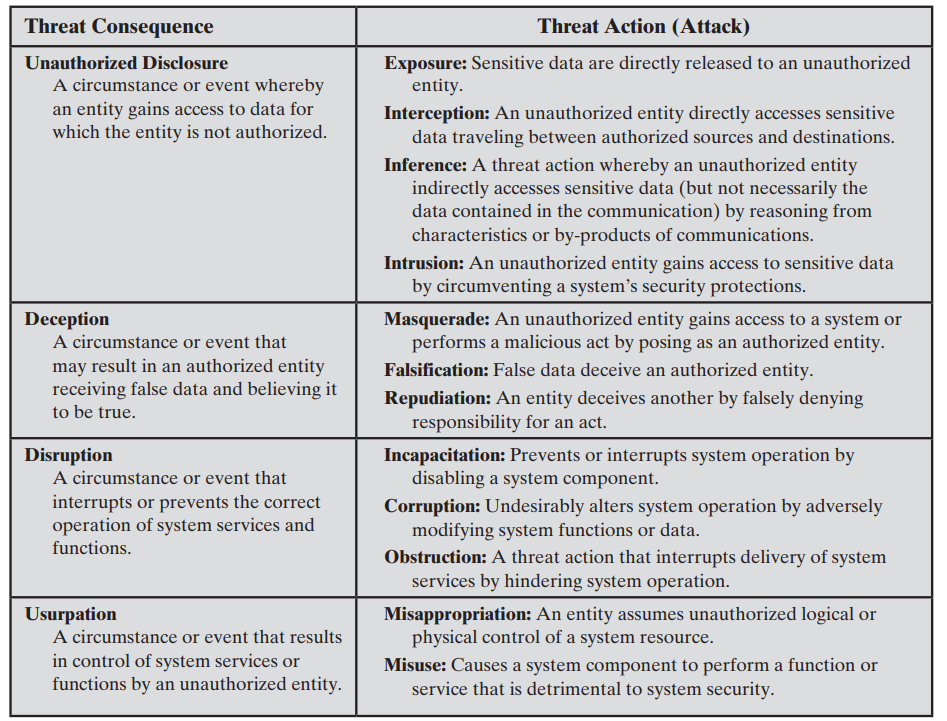
\includegraphics[width=14cm, keepaspectratio]{bistarelli/img/cap_1/tabella_minacce.png}
	\caption{Conseguenze delle minacce e azioni che le causano }\label{fig:tabella_minacce}
\end{figure}

La tabella \ref{fig:tabella_minacce} basata su RFC 4949, descrive quattro tipi di conseguenze ed elenca i tipi di attacchi che risultano in ciascuna conseguenza. 

La divulgazione non autorizzata (Unauthorized disclosure) è una minaccia alla riservatezza. I seguenti tipi di attacchi possono portare a queste conseguenze

\begin{itemize}
    \item \textbf{Esposizione}: quando un insider rilascia intenzionalmente informazioni sensibili a un estraneo, come ad esempio i numeri di carta di credito. Può anche essere il risultato di un errore umano, hardware o software, che si traduce nell'azione da parte di un'entità di avere l'accesso non autorizzato di dati sensibili. Ce ne sono stati numerosi casi di questo, come le università che pubblicano accidentalmente le informazioni confidenziali degli studenti sul Web.
    \item \textbf{Intercettazione}: l'intercettazione è un attacco comune nel contesto delle comunicazioni. Su una rete locale condivisa (LAN), come una LAN wireless o a broadcast Ethernet, qualsiasi dispositivo collegato alla LAN può ricevere una copia dei pacchetti destinati a un altro dispositivo. Su Internet, un determinato hacker può accedere al traffico di posta elettronica e ad altri trasferimenti di dati. Tutte queste situazioni possono portare all'accesso non autorizzato ai dati.
    \item \textbf{Inferenza}: un esempio di inferenza è noto come analisi del traffico, in cui un avversario è in grado di ottenere informazioni osservando l'andamento del traffico una rete, come la quantità di traffico tra particolari coppie di host sulla rete. Un altro esempio è l'inferenza di informazioni dettagliate da un database di un utente che ha solo un accesso limitato, questo è realizzato da query ripetute i cui risultati combinati consentono l'inferenza.
    \item \textbf{Intrusione}: un esempio di intrusione è un avversario che ottiene l'accesso non autorizzato a dati sensibili superando le protezioni di controllo degli accessi del sistema.
\end{itemize}

L'inganno (Deception) è una minaccia per l'integrità del sistema o per l'integrità dei dati. I seguenti tipi di attacchi possono portare a queste conseguenze:
\begin{itemize}
    \item \textbf{Masquerade}: un esempio di masquerade è un tentativo di accesso a un sistema  da parte di un utente non autorizzato spacciandosi per uno autorizzato, questo può succedere se l'utente non autorizzato conosce l'ID di accesso e la password di un altro utente. Un altro esempio è la logica dannosa (malicious logic), come un cavallo di Troia, che appare per eseguire una funzione utile o desiderabile, ma in realtà ottiene l'accesso non autorizzato alle risorse di sistema o induce un utente a eseguire altre logiche dannose.
    \item \textbf{Falsificazione}: si riferisce all'alterazione o sostituzione di dati validi o all'introduzione di dati falsi in un file o database. Ad esempio, uno studente può alterare i suoi voti su un database scolastico.
    \item \textbf{Ripudio}: in questo caso, un utente nega l'invio di dati o nega di ricevere o possedere i dati.
\end{itemize}

L'interruzione (Disruption) è una minaccia alla disponibilità o all'integrità del sistema. I seguenti tipi di attacchi possono portare a queste conseguenze:
\begin{itemize}
    \item \textbf{Incapacità}: questo è un attacco alla disponibilità del sistema. Ciò potrebbe verificarsi come risultato della distruzione fisica o del danneggiamento dell'hardware del sistema. Più tipicamente, un software dannoso, come Trojan, virus o worm, potrebbero operarein modo tale da disabilitare un sistema o alcuni dei suoi servizi.
    \item \textbf{Corruzione}: questo è un attacco all'integrità del sistema. Un Software dannoso in questo contesto potrebbe funzionare in modo tale che le risorse di sistema o i servizi funzionino in modo non intenzionale. Oppure un utente potrebbe ottenere l'accesso non autorizzato a un sistema e modificarne alcune funzioni. Un esempio di quest'ultimo è un posizionamento di una logica backdoor (backdoor logic) nel sistema per fornire il successivo accesso al sistema stesso e alle sue risorse con una procedura diversa da quella abituale.
    \item \textbf{Ostruzione}: un modo per ostacolare il funzionamento del sistema è interferire con le comunicazioni disabilitando i collegamenti di comunicazione o alterando la comunicazione delle informazioni di controllo. Un altro modo è sovraccaricare il sistema mettendo un carico in eccesso sul traffico di una comunicazione o sulle risorse di elaborazione.
\end{itemize}

L'usurpazione (Usurpation) è una minaccia per l'integrità del sistema. I seguenti tipi di attacchi possono portare a queste conseguenze:
\begin{itemize}
    \item \textbf{Appropriazione indebita}: può includere il furto del servizio. Un esempio è un attacco Denial of Service distribuito, quando il software dannoso è installato su degli host da utilizzare come piattaforme per avviare il traffico verso un host di destinazione. In questo caso, il software maligno fa uso non autorizzato delle risorse del processore e del sistema operativo.
    \item \textbf{Uso improprio}: l'uso improprio può verificarsi per mezzo di una malicious logic o di un hacker che ha ottenuto un accesso non autorizzato a un sistema. In entrambi i casi, le funzioni di sicurezza possono essere disabilitate o contrastate.
\end{itemize}

\subsection{Asset e minacce}
Le risorse di un sistema informatico possono essere classificate come hardware, software, dati, linee e reti di comunicazione. In questa sottosezione li descriviamo brevemente e mettendoli in relazione con i concetti di integrità, riservatezza e
disponibilità. 

\begin{figure}[H]
	\centering
    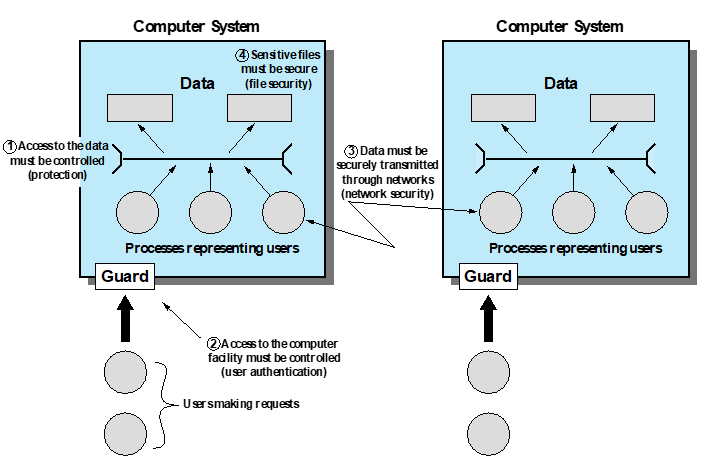
\includegraphics[width=14cm, keepaspectratio]{bistarelli/img/cap_1/asset_sec.png}
	\caption{ Scopo della sicurezza informatica.}\label{fig:asset_sec}
\end{figure}

\paragraph{Hardware.} Una delle principali minacce per l'hardware  del computer è la minaccia alla disponibilità. L'hardware è il più vulnerabile agli attacchi e il meno suscettibile ai controlli automatizzati. Le minacce includono danni accidentali e deliberati alle apparecchiature così come il furto. La proliferazione di personal computer e workstation e l'uso diffuso delle LAN aumenta il potenziale di perdite in quest'area. Il furto delle unità USB può portare alla perdita di riservatezza. Le misure di sicurezza fisiche e amministrative sono necessarie per far fronte a queste minacce.


\paragraph{Software.} Il software include il sistema operativo, le utilità e l'applicazione programmi. Una delle principali minacce al software è un attacco alla disponibilità. Il Software, in particolare quello applicativo, è spesso facile da eliminare. Il software può anche essere modificato o danneggiato per renderlo inutilizzabile. Un'attenta gestione della configurazione del software, che include il mantenere dei backup della versione più recente, può mantenere una disponibilità alta. Un problema più difficile da affrontare è la modifica del software che si ha in un programma il quale funziona ancora ma che si comporta in modo diverso rispetto a prima,
questa è una minaccia per l'integrità/autenticità. Rientrano in questa categoria i virus informatici e i relativi attacchi. Un ultimo problema è la protezione contro la pirateria del software. Sebbene siano disponibili alcune contromisure, in linea di massima il problema di copie non autorizzate del software non è stata risolta.

\paragraph{Data.}  Un  problema molto più diffuso è la sicurezza dei dati, che coinvolge file e altre forme di dati controllati da individui, gruppi e organizzazioni aziendali.

I problemi di sicurezza relativi ai dati sono ampi e comprendono disponibilità, segretezza e integrità. In caso di disponibilità, la preoccupazione è con la distruzione di file di dati, che può verificarsi accidentalmente o intenzionalmente. 
Una preoccupazione evidente per la segretezza è la lettura non autorizzata di file di dati o database, e quest'area è stata forse oggetto di ulteriori ricerche e sforzi rispetto a qualsiasi altro settore della sicurezza informatica. Una minaccia meno ovvia alla segretezza comporta l'analisi dei dati e si manifesta nell'utilizzo delle cosiddette banche dati statistiche, che forniscono informazioni di sintesi o aggregate. Presumibilmente, l'esistenza delle informazioni aggregate non minacciano la privacy delle persone coinvolte. Tuttavia, con la crescita dell'uso delle banche dati statistiche, c'è un rischio crescente per la divulgazione di informazioni personali. In sostanza, le caratteristiche di un individuo possono essere identificate attraverso un'analisi attenta. Ad esempio, se una tabella registra l'aggregato dei redditi degli intervistati A, B, C e D e un altro registra l'aggregato dei redditi di A, B, C, D ed E, la differenza tra i due aggregati sarebbe il reddito di E. Questo problema è esasperato dal desiderio crescente di combinare set di dati. In molti casi, abbinando diversi set di dati per coerenza tra i diversi livelli di aggregazione è necessario l'accesso alle singole unità. Pertanto, le singole unità, che sono oggetto di problemi di privacy, sono disponibili in varie fasi del trattamento dei set di dati. 
Infine, l'integrità dei dati è una delle principali preoccupazioni nella maggior parte delle installazioni.Le modifiche ai file di dati possono avere conseguenze che vanno da minori a disastrose.

\subsection{Attacchi passivi e attivi}
Gli attacchi alla sicurezza della rete possono essere classificati
come attacchi passivi e attacchi attivi. Un attacco passivo tenta di imparare o fare
uso delle informazioni del sistema, ma non influisce sulle risorse di quest'ultimo. Un attacco attivo tenta di alterare le risorse di sistema o di influenzare il loro funzionamento.

\subsubsection{Attacchi passivi}
Gli \textbf{attacchi passivi} generalmente riguardano l'intercettazione o il monitoraggio di trasmissioni di dati. L'obiettivo dell'attaccante è ottenere le informazioni che vengono trasmesse. Due tipi di attacchi passivi sono il rilascio del contenuto dei messaggi e dell'analisi del traffico.

\paragraph{Rilascio dei contenuti di un messaggio} Il \textbf{rilascio dei contenuti} del messaggio è facilmente comprensibile. Una conversazione telefonica, un messaggio di posta elettronica e un file trasferito possono contenere dati sensibili o informazioni confidenziali. Vorremmo impedire a un avversario di imparare il contenuto di queste trasmissioni.

\paragraph{Analisi del traffico.} Un secondo tipo di attacco passivo, \textbf{l'analisi del traffico}, è più sottile. Supponiamo che noi abbiamo un modo per mascherare il contenuto dei messaggi o altre informazioni del traffico di dati, in modo che gli oppositori, anche se hanno catturato il messaggio, non possono estrarre le informazioni dal messaggio. La tecnica comune per mascherare i contenuti è la crittografia. Anche se disponiamo di una protezione crittografica, un avversario potrebbe comunque essere in grado di osservare lo schema di questi messaggi. L'avversario potrebbe determinare la posizione e l'identità degli host nella comunicazione e potrebbe osservare la frequenza e la lunghezza dei messaggi scambiati. Queste informazioni potrebbero essere utili per indovinare la natura della comunicazione che stava avvenendo.

Gli attacchi passivi sono molto difficili da rilevare perché non coinvolgono alterazione dei dati. In genere, il traffico dei messaggi viene inviato e ricevuto in un modo apparentemente normale e né il mittente né il destinatario sono consapevoli che una terza parte ha letto i messaggi o osservato l'andamento del traffico. Tuttavia, è possibile prevenire il successo di questi attacchi, di solito mediante crittografia. Pertanto, l'enfasi nell'affrontare gli attacchi passivi è sulla prevenzione piuttosto che il rilevamento.

\subsubsection{Attacchi attivi}
Gli attacchi attivi comportano alcune modifiche del flusso di dati o la creazione
di un falso flusso, esso può essere suddiviso in quattro categorie: replay, masquerade, modifica dei messaggi e denial of service.

\paragraph{Replay.} Il replay comporta l'acquisizione passiva di un'unità di dati e la sua successiva ritrasmissione per produrre un effetto non autorizzato.


\paragraph{Masquerade.} Una masquerade ha luogo quando un'entità finge di essere un'entità diversa. Un attacco di questo tipo di solito include una delle altre forme di attacco attivo. Per esempio, le sequenze di autenticazione possono essere catturate e riprodotte dopo che è avvenuta una sequenza di autenticazione valida, abilitando così un'entità autorizzata con pochi privilegi a ottenere privilegi extra impersonando un'entità che dispone di tali privilegi.

\paragraph{Modifica di un messaggio.} La modifica dei messaggi significa semplicemente che una parte di un legittimo messaggio è alterato, o che i messaggi sono ritardati o riordinati, per produrre un effetto non autorizzato. Ad esempio, un messaggio che afferma: "Consenti a John Smith di leggere dati di file riservati" viene modificato per dire "Consenti a Fred Brown di leggere dati di file riservati".

\paragraph{DOS.} La negazione del servizio impedisce o inibisce il normale utilizzo o gestione delle strutture di comunicazione. Questo attacco può avere un obiettivo specifico, per esempio un'entità può sopprimere tutti i messaggi diretti a una particolare destinazione (ad esempio, la sicurezza del servizio di audit). Un'altra forma di rifiuto del servizio è l'interruzione di un'intera rete, o disabilitando la rete o sovraccaricandola di messaggi in modo da degradarne le prestazioni.

Gli attacchi attivi presentano le caratteristiche opposte degli attacchi passivi. Invece gli attacchi passivi sono difficili da rilevare, sono disponibili misure per prevenirli con successo. D'altra parte, è abbastanza difficile prevenire assolutamente gli attacchi attivi, perché per farlo richiederebbe la protezione fisica di tutte le strutture e i percorsi di comunicazione in ogni momento. Invece, l'obiettivo è rilevarli e riprendersi da qualsiasi disservizio o ritardi da essi causati. Poiché il rilevamento ha un effetto deterrente, esso può anche contribuire alla prevenzione.

\subsection{Requisiti di sicurezza} 
Esistono diversi modi per classificare e caratterizzare le contromisure che possono essere utilizzate per ridurre le vulnerabilità e affrontare le minacce alle risorse di sistema. In questa sottosezione, vediamo contromisure in termini di requisiti funzionali, e seguiamo la classificazione definita in FIPS 200. Questo standard enumera 17 aree relative alla sicurezza con riguardo alla protezione della riservatezza, dell'integrità e della disponibilità delle informazioni di sistemi e le informazioni elaborate, archiviate e trasmesse da tali sistemi.
\begin{enumerate}
    \item \textbf{Accesso controllato}: limitare l'accesso al sistema informativo agli utenti autorizzati, ai processi che agiscono per conto degli utenti autorizzati, o ai dispositivi (inclusi altri sistemi informativi) e alle tipologie di transazioni e funzioni che gli utenti autorizzati possono esercitare.
    \item \textbf{Consapevolezza e Formazione}: garantire che i gestori e gli utenti dei sistemi informativi organizzativi siano consapevole dei rischi per la sicurezza associati alle proprie attività e delle leggi, dei regolamenti e delle politiche applicabili relativi alla sicurezza dei sistemi informativi organizzativi e  garantire che il personale sia adeguatamente addestrato a svolgere i compiti e le responsabilità assegnate in materia di sicurezza delle informazioni.
    \item \textbf{Audit e responsabilità}: creare, proteggere e conservare i record di audit del sistema informativo per consentire il monitoraggio, l'analisi, l'indagine e la segnalazione di atti illeciti, non autorizzati o di attività non appropriate del sistema informativo. Garantire inoltre che le azioni dei singoli individui  nel sistema possano essere ricondotte in modo univoco a tali utenti in modo che possano essere ritenuti responsabili di esse.
    \item \textbf{Certificazione, accreditamento e valutazioni di sicurezza}: valutare periodicamente i controlli di sicurezza nei sistemi informativi organizzativi per determinare se i controlli sono efficaci nella loro applicazione. Sviluppare e attuare piani d'azione volti a correggere le carenze e ridurre o eliminare le vulnerabilità in questi sistemi. Autorizzare l'esercizio dei sistemi informativi organizzativi ed eventuali connessioni associate a questi. Monitorare continuamente i controlli di sicurezza del sistema informativo  per garantire la continua efficacia di essi.
    \item \textbf{Gestione della configurazione}: stabilire e mantenere le configurazioni di base e gli inventari dei sistemi (inclusi hardware, software, firmware e documentazione) durante i rispettivi cicli di vita di sviluppo del sistema. Stabilire e far rispettare le impostazioni di configurazione di sicurezza per i prodotti informatici utilizzati nei sistemi.
    \item \textbf{Pianificazione di emergenza}: stabilire, mantenere e implementare piani di risposta alle emergenze, operazioni di backup, e il ripristino post-disastro per i sistemi in modo da garantire la disponibilità di risorse informative critiche e continuità operativa in situazioni di emergenza.
    \item \textbf{Identificazione e autenticazione}: identificare gli utenti del sistema, i processi che agiscono per conto degli utenti o dei dispositivi e autenticare (o verificare) le identità di tali utenti, processi o dispositivi, come prerequisito per consentire l'accesso ai sistemi.
    \item \textbf{Risposta all'incidente}: stabilire una capacità operativa di gestione degli incidenti per le informazioni organizzative dei sistemi che includono un'adeguata preparazione, rilevamento, analisi, contenimento, recupero e un controllo delle attività di risposta dell'utente. Tracciare, documentare e segnalare gli incidenti ai funzionari appropriati e/o alle autorità.
    \item \textbf{Manutenzione}: eseguire la manutenzione periodica e tempestiva dei sistemi, fornire controlli efficaci sugli strumenti, sulle tecniche, sui meccanismi e sul personale utilizzato per condurre una manutenzione del sistema informativo.
    \item \textbf{Protezione dei media}: proteggere i media dei sistemi, sia cartacei che digitali, limitare l'accesso alle informazioni dei media agli utenti autorizzati e sanificare o distruggere prima i supporti del sistema informativo prima dello smaltimento o del rilascio per il riutilizzo.
    \item \textbf{Protezione fisica e ambientale}: limitare l'accesso fisico dei soggetti autorizzati ai sistemi informativi, alle apparecchiature e ai rispettivi ambienti operativi. Proteggere l'impianto fisico e l' infrastruttura di supporto per i sistemi. Fornire utilità di supporto per i sistemi informativi e proteggere quest'ultimi dai rischi ambientali fornendo adeguati controlli ambientali alle strutture che li contengono.
    \item \textbf{Pianificazione}: sviluppare, documentare, aggiornare periodicamente e implementare piani di sicurezza per le informazioni organizzative dei sistemi che descrivono i controlli di sicurezza esistenti o previsti e le regole di comportamento dei soggetti che accedono ai sistemi.
    \item \textbf{Sicurezza del personale}: garantire che le persone che occupano posizioni di responsabilità all'interno delle organizzazioni (compresi i fornitori di servizi di terze parti) siano affidabili e soddisfino i criteri di sicurezza stabiliti per quelle posizioni. Garantire che le informazioni organizzative e i sistemi informativi siano protetti durante e dopo le azioni del personale quali licenziamenti e trasferimenti. Applicare sanzioni formali per il personale che non fa rispettare le politiche e le procedure di sicurezza dell'organizzazione.
    \item \textbf{Valutazione del rischio}: valutare periodicamente il rischio per le operazioni organizzative (inclusi missioni, funzioni, immagine o reputazione), risorse organizzative e individui, risultanti dal funzionamento del sistema e il relativo trattamento, archiviazione o trasmissione di informazioni organizzative.
    \item \textbf{Acquisizione di sistemi e servizi}: Allocare risorse sufficienti per proteggere adeguatamente l'organizzazione dei sistemi. Impiegare processi del ciclo di vita dello sviluppo del sistema che incorporano considerazioni sulla sicurezza. Imporre limitazioni all'utilizzo e all'installazione del software e garantire che i fornitori di terze parti adottino adeguate misure di sicurezza per proteggere le informazioni, le applicazioni e/o i servizi "esternalizzati" dall'organizzazione.
    \item \textbf{Protezione del sistema e delle comunicazioni}: monitorare, controllare e proteggere le comunicazioni organizzative (vale a dire, le informazioni trasmesse o ricevute dai sistemi) ai confini esterni e interni. Impiegare progetti "architettonici", sviluppo software tecniche e principi di ingegneria dei sistemi che promuovono un'efficace sicurezza delle informazioni all'interno di dei sistemi organizzativi.
    \item \textbf{Integrità del sistema e delle informazioni}: identificare, segnalare e correggere le informazioni e le falle del sistema in modo tempestivo. Fornire protezione da codice dannoso in posizioni appropriate all'interno del sistema organizzativo e monitorare gli avvisi di sicurezza del sistema informativo e adottare le azioni appropriate in risposta.
\end{enumerate}
    %...
    \bibliographystyle{plainnat}
    \newpage
    % Opzionale
    %\listoffigures
    %\listoftables
    \bibliography{bibliografia}
    
\end{document}
